%%%%%% Run at command line, run
%%%%%% xelatex grad-sample.tex 
%%%%%% for a few times to generate the output pdf file
\documentclass[12pt,oneside,openright,a4paper]{cpe-thai-project}


\usepackage{polyglossia}
\setdefaultlanguage{thai}
\setotherlanguage{english}
\newfontfamily\thaifont[Script=Thai,Scale=1.23]{TH Sarabun New}
\defaultfontfeatures{Mapping=tex-text,Scale=1.23,LetterSpace=0.0}
\setmainfont[Scale=1.23,LetterSpace=0,WordSpace=1.0,FakeStretch=1.0,Mapping=tex-text]{TH Sarabun New}
\XeTeXlinebreaklocale "th"	
\XeTeXlinebreakskip = 0pt plus 0pt
\emergencystretch=10pt

%%%%%%%%%%%%%%%%%%%%%%%%%%%%%%%%%%%%%%%%%%%%%%%%%%%%%%%%%%%%%%%%%%%
% Customize below to suit your needs 
% The ones that are optional can be left blank. 
%%%%%%%%%%%%%%%%%%%%%%%%%%%%%%%%%%%%%%%%%%%%%%%%%%%%%%%%%%%%%%%%%%%
% First line of title
\def\disstitleone{Easy room web application with generative Interior design AI using Stable Diffusion Model}   
% Second line of title
\def\disstitletwo{เว็บแอปพลิเคชันสำหรับผู้ที่ต้องการออกแบบภายในโดยปัญญาประดิษฐ์ด้วย Stable Diffusion}   
% Your first name and lastname
\def\dissauthor{Mr. Phuettipol Jitjaroenkit}   % 1st member
%%% Put other group member names here ..
\def\dissauthortwo{Mr. Wichayut  Chuaychukul}   % 2nd member (optional)
\def\dissauthorthree{Mr. Thanpisit Pisitpon}   % 3rd member (optional)


% The degree that you're persuing..
\def\dissdegree{Bachelor of Engineering} % Name of the degree
\def\dissdegreeabrev{B.Eng} % Abbreviation of the degree
\def\dissyear{2023}                   % Year of submission
\def\thaidissyear{2566}               % Year of submission (B.E.)

%%%%%%%%%%%%%%%%%%%%%%%%%%%%%%%%%%%%%%%%%%%%
% Your project and independent study committee..
%%%%%%%%%%%%%%%%%%%%%%%%%%%%%%%%%%%%%%%%%%%%
\def\dissadvisor{Dr. Taweechai Nusantiwong}  % Advisor
%%% Leave it empty if you have no Co-advisor
\def\disscoadvisor{}  % Co-advisor
\def\disscoadvisortwo{}  % Co-advisor
\def\disscommitteetwo{}  % 3rd committee member (optional)
\def\disscommitteethree{Asst.Prof. Committee3, Ph.D.}   % 4th committee member (optional) 
\def\disscommitteefour{}    % 5th committee member (optional) 

\def\worktype{Project} %%  Project or Independent study
\def\disscredit{3}   %% 3 credits or 6 credits


\def\fieldofstudy{Computer Engineering} 
\def\department{Computer Engineering} 
\def\faculty{Engineering}

\def\thaifieldofstudy{วิศวกรรมคอมพิวเตอร์} 
\def\thaidepartment{วิศวกรรมคอมพิวเตอร์} 
\def\thaifaculty{วิศวกรรมศาสตร์}
 
\def\appendixnames{Appendix} %%% Appendices or Appendix

\def\thaiworktype{ปริญญานิพนธ์} %  Project or research project % 
\def\thaidisstitleone{Easy room web application with generative Interior design AI using Stable Diffusion Model}   
\def\thaidisstitletwo{เว็บแอปพลิเคชันสำหรับผู้ที่ต้องการออกแบบภายในโดยปัญญาประดิษฐ์ด้วย Stable Diffusion}
\def\thaidissauthor{นายพฤฒิพล จิตรเจริญกิจ}
\def\thaidissauthortwo{นายวิชยุฒม์ ช่วยชูกูล} %Optional
\def\thaidissauthorthree{นายธัญพิสิษฐ์ พิสิฐพล} %Optional

\def\thaidissadvisor{ดร.ทวีชัย นันทวิสุทธิวงศ์}
%% Leave this empty if you have no co-advisor
\def\thaidisscoadvisor{} %Optional
\def\thaidisscoadvisortwo{} %Optional
\def\thaidissdegree{วิศวกรรมศาสตรบัณฑิต}

% Change the line spacing here...
\linespread{1.15}

%%%%%%%%%%%%%%%%%%%%%%%%%%%%%%%%%%%%%%%%%%%%%%%%%%%%%%%%%%%%%%%%
% End of personal customization.  Do not modify from this part 
% to \begin{document} unless you know what you are doing...
%%%%%%%%%%%%%%%%%%%%%%%%%%%%%%%%%%%%%%%%%%%%%%%%%%%%%%%%%%%%%%%%


%%%%%%%%%%%% Dissertation style %%%%%%%%%%%
%\linespread{1.6} % Double-spaced  
%%\oddsidemargin    0.5in
%%\evensidemargin   0.5in
%%%%%%%%%%%%%%%%%%%%%%%%%%%%%%%%%%%%%%%%%%%
%\renewcommand{\subfigtopskip}{10pt}
%\renewcommand{\subfigbottomskip}{-5pt} 
%\renewcommand{\subfigcapskip}{-6pt} %vertical space between caption
%                                    %and figure.
%\renewcommand{\subfigcapmargin}{0pt}

\renewcommand{\topfraction}{0.85}
\renewcommand{\textfraction}{0.1}

\newtheorem{theorem}{Theorem}
\newtheorem{lemma}{Lemma}
\newtheorem{corollary}{Corollary}

\def\QED{\mbox{\rule[0pt]{1.5ex}{1.5ex}}}
\def\proof{\noindent\hspace{2em}{\itshape Proof: }}
\def\endproof{\hspace*{\fill}~\QED\par\endtrivlist\unskip}
%\newenvironment{proof}{{\sc Proof:}}{~\hfill \blacksquare}
%% The hyperref package redefines the \appendix. This one 
%% is from the dissertation.cls
%\def\appendix#1{\iffirstappendix \appendixcover \firstappendixfalse \fi \chapter{#1}}
%\renewcommand{\arraystretch}{0.8}
%%%%%%%%%%%%%%%%%%%%%%%%%%%%%%%%%%%%%%%%%%%%%%%%%%%%%%%%%%%%%%%%
%%%%%%%%%%%%%%%%%%%%%%%%%%%%%%%%%%%%%%%%%%%%%%%%%%%%%%%%%%%%%%%%

\usepackage{ragged2e}
\begin{document}

\pdfstringdefDisableCommands{%
\let\MakeUppercase\relax
}

\begin{center}
  
\includegraphics[width=2.8cm]{image/logo.jpg}
\end{center}
\vspace*{-1cm}

\maketitlepage
\makesignaturepage 

%%%%%%%%%%%%%%%%%%%%%%%%%%%%%%%%%% English abstract %%%%%%%%%%%%%%%%%%%%%%%%%%%%%%%
\abstract

In a multihop ad hoc network, the interference among nodes is
  reduced to maximize the throughput by using a smallest transmission
  range that still preserve the network connectivity. However, most
  existing works on transmission range control focus on the
  connectivity but lack of results on the throughput performance. This
  paper analyzes the per-node saturated throughput of an IEEE 802.11b
  multihop ad hoc network with a uniform transmission range. Compared
  to simulation, our model can accurately predict the per-node
  throughput.  The results show that the maximum achievable per-node
  throughput can be as low as 11\% of the channel capacity in a normal
  set of $\alpha$ operating parameters independent of node density. However, if
  the network connectivity is considered, the obtainable throughput
  will reduce by as many as 43\% of the maximum throughput. 

\begin{flushleft}
\begin{tabular*}{\textwidth}{@{}lp{0.8\textwidth}}
\textbf{Keywords}: & Multihop ad hoc networks / Topology control / Single-Hop Throughput
\end{tabular*}
\end{flushleft}
\endabstract

%%%%%%%%%%%%%%%%%%%%%%%%%%%%%%%%%%%%%%%%%%%%%%%%%%%%%%%%%%%%%%
%%%%%%%%%% Thai abstract here %%%%%%%%%%%%%%%%%%%%%%%%%%%%%%%%%
%%%%%%%%%%%%%%%%%%%%%%%%%%%%%%%%%%%%%%%%%%%%%%%%%%%%%%%%%%%%%%
% {\newfontfamily\thaifont{TH Sarabun New:script=thai}[Scale=1.3]
% \XeTeXlinebreaklocale "th_TH"	
% \thaifont
\thaiabstract

เซ็นเซอร์ เอ็กซ์เพรสรองรับคอนเซปต์สหัสวรรษเมจิก อิ่มแปร้ เฟรชชี่ ชาร์ปเช็งเม้งคลาสสิก แพตเทิร์น แอลมอนด์ เพลซว้อยก๊วน ซาร์ดีนซี้เนิร์สเซอรีอีสต์ สเตเดียมเพียบแปร้โอ้ยแคมปัส จัมโบ้ช็อตแมคเคอเรลอึ๋ม สตริง แมกกาซีนสตริงผ้าห่ม ฮัลโหล ยิม รอยัลตี้

\begin{flushleft}
\begin{tabular*}{\textwidth}{@{}lp{0.8\textwidth}}
 & \\

\textbf{คำสำคัญ}: & การชุบเคลือบด้วยไฟฟ้า / การชุบเคลือบผิวเหล็ก /  เคลือบผิวรังสี
\end{tabular*}
\end{flushleft}
\endabstract

%}

%%%%%%%%%%%%%%%%%%%%%%%%%%%%%%%%%%%%%%%%%%%%%%%%%%%%%%%%%%%%
%%%%%%%%%%%%%%%%%%%%%%% Acknowledgments %%%%%%%%%%%%%%%%%%%%
%%%%%%%%%%%%%%%%%%%%%%%%%%%%%%%%%%%%%%%%%%%%%%%%%%%%%%%%%%%%
\preface
ขอบคุณอาจารย์ที่ปรึกษา กรรมการ พ่อแม่พี่น้อง และเพื่อนๆ คนที่ช่วยให้งานสำเร็จ ตามต้องการ

%%%%%%%%%%%%%%%%%%%%%%%%%%%%%%%%%%%%%%%%%%%%%%%%%%%%%%%%%%%%%
%%%%%%%%%%%%%%%% ToC, List of figures/tables %%%%%%%%%%%%%%%%
%%%%%%%%%%%%%%%%%%%%%%%%%%%%%%%%%%%%%%%%%%%%%%%%%%%%%%%%%%%%%
% The three commands below automatically generate the table 
% of content, list of tables and list of figures
\tableofcontents                    
\listoftables
\listoffigures                      

%%%%%%%%%%%%%%%%%%%%%%%%%%%%%%%%%%%%%%%%%%%%%%%%%%%%%%%%%%%%%%
%%%%%%%%%%%%%%%%%%%%% List of symbols page %%%%%%%%%%%%%%%%%%%
%%%%%%%%%%%%%%%%%%%%%%%%%%%%%%%%%%%%%%%%%%%%%%%%%%%%%%%%%%%%%%
% You have to add this manually..
\listofsymbols
\begin{flushleft}
\begin{tabular}{@{}p{0.07\textwidth}p{0.7\textwidth}p{0.1\textwidth}}
\textbf{SYMBOL}  & & \textbf{UNIT} \\[0.2cm]
$\alpha$ & Test variable\hfill & m$^2$ \\
$\lambda$ & Interarival rate\hfill &  jobs/second\\
$\mu$ & Service rate\hfill & jobs/second\\
\end{tabular}
\end{flushleft}
%%%%%%%%%%%%%%%%%%%%%%%%%%%%%%%%%%%%%%%%%%%%%%%%%%%%%%%%%%%%%%
%%%%%%%%%%%%%%%%%%%%% List of vocabs & terms %%%%%%%%%%%%%%%%%
%%%%%%%%%%%%%%%%%%%%%%%%%%%%%%%%%%%%%%%%%%%%%%%%%%%%%%%%%%%%%%
% You also have to add this manually..
\listofvocab
\begin{flushleft}
\begin{tabular}{@{}p{1in}@{=\extracolsep{0.5in}}p{0.73\textwidth}}
Test &  Lorem ipsum dolor sit amet, consectetur adipiscing elit. Nullam non condimentum purus. Pellentesque sed augue sapien. In volutpat quis diam laoreet suscipit. Curabitur fringilla sem nisi, at condimentum lectus consequat vitae.\\
MANET & Mobile Ad Hoc Network 
\end{tabular}
\end{flushleft}

%\setlength{\parskip}{1.2mm}

%%%%%%%%%%%%%%%%%%%%%%%%%%%%%%%%%%%%%%%%%%%%%%%%%%%%%%%%%%%%%%%
%%%%%%%%%%%%%%%%%%%%%%%% Main body %%%%%%%%%%%%%%%%%%%%%%%%%%%%
%%%%%%%%%%%%%%%%%%%%%%%%%%%%%%%%%%%%%%%%%%%%%%%%%%%%%%%%%%%%%%%

%%%%%%%%%%%%%%%%%%%%%%%%%%%%%%%%%% บทที่  1 %%%%%%%%%%%%%%%%%%%%%%%%%%%%%%%%%%%

\chapter{}

\section{ที่มาและความสำคัญ}
\hspace {18pt}Artificial Intelligence (AI) หรือ ปัญญาประดิษฐ์ เป็นเทคโนโลยีที่มีความสำคัญ และกำลังได้รับความนิยมเป็นอย่างมาก เทคโนโลยี AI ในช่วงแรกจะใช้หลักการ Machine Learning คือการให้คอมพิวเตอร์เรียนรู้ด้วยตนเอง ผ่านข้อมูลที่มันได้รับ เทคโนโลยีที่เหนือจาก Machine Learning ไปอีกระดับคือ Deep Learning  ซึ่งเป็น Machine Learning ที่ลอกเลียนแบบโครงสร้างของระบบประสาทของมนุษย์ที่เรียกว่า Neural Network มาใช้ในการพัฒนาความฉลาดของ AI โดยการเทรน(train) หรือให้ Neural Network เรียนรู้จากข้อมูลมหาศาล ซึ่งในสมัยก่อนการหาข้อมูลมาเทรน AI ค่อนข้างยากและใช้เวลานาน แต่ในปัจจุบันข้อมูลสามารถค้นหาได้ง่ายและมีอยู่มากมายอินเตอร์เน็ต รวมไปถึงเทคโนโลยีอื่นๆเช่น หน่วยประมวลผลกราฟิก (GPU) ที่มีส่วนช่วยให้ใช้เวลาน้อยลงในการเทรน AI จึงทำให้ปัจจุบันพบ AI มากมายและมีความสามารถมากกว่าสมัยก่อน เช่น เทคโนโลยีรถยนต์ไร้คนขับ Generative AI ที่สามารถช่วยสร้างผลลัพธ์ในรูปแบบต่างเช่น ข้อความ เสียง รูปภาพ วิดีโอ จากคำสั่งของมนุษย์ที่บอกให้ช่วยสร้างหรือให้ช่วยหาคำตอบให้ เช่น ChatGPT \cite{chatgpt} Midjourney [2] Dall ·E [3] Stable Diffusion [4] ด้วย Generative AI เหล่านี้ สามารถแบ่งเบาภาระของมนุษย์ได้อย่างมาก โดย Midjourney Dall·E Stable diffusion สามารถสร้างรูปภาพผ่าน Prompt หรือคำสั่งในรูปแบบข้อความ
 \par \hspace {18pt} 
จากที่กล่าวมาข้างต้นด้วยความสามารถของ AI เหล่านี้จึงเกิดความคิดที่จะใช้มันการออกแบบห้องซึ่งจากการสำรวจทางอินเตอร์เน็ตพบว่า มีเว็บไซต์ที่ใช้ AI ในการออกแบบห้องอยู่พอสมควรในหลายรูปแบบ เช่น 1. ใช้เปลี่ยนสไตล์ของห้องโดยจะรับข้อมูลเป็น รูปภาพของห้องและสไตล์ของห้องที่อยากให้เป็น 2. ใช้ในการออกแบบภายใน รับข้อมูลเป็นสไตล์ของห้องและชนิดของห้อง ซึ่งในบางเว็บไซต์มีฟีเจอร์ที่สามารถใช้ Google Lens [5] ในการหาผลิตภัณฑ์ที่ใช้ในรูปภาพ ซึ่งผลลัพธ์ที่ได้จาก Google Lens จะเป็นผลิตภัณฑ์ที่ใกล้เคียง มีบางผลิตภัณฑ์ที่หาซื้อได้ผ่าน Amazon หรือ IKEA
\par  \hspace {18pt}
คณะผู้จัดทำมีความเห็นว่าเครื่องมืออำนวยความสะดวกด้านการออกแบบภายในเหล่านี้ อาจไม่ตอบโจทย์ผู้ใช้งานชาวไทยเท่าที่ควรเช่น เฟอร์นิเจอร์ ของตกแต่ง วัสดุต่างๆอาจไม่มีตัวแทนจำหน่ายในประเทศไทยจึงทำให้สั่งซื้อได้ยาก และไม่สามารถประเมินราคาค่าใช้จ่าย จากปัญหาที่กล่าวไว้ข้างต้นทำให้คณะผู้จัดทำคิดริเริ่มที่จะพัฒนาเว็บแอปพลิเคชันที่มี AI ในการออกแบบภายในเพื่ออำนวยความสะดวกให้กับผู้ใช้ชาวไทยโดยจะใช้ผลิตภัณฑ์เฟอร์นิเจอร์ ของตกแต่งที่สามารถหาซื้อได้ที่ประเทศไทย สามารถระบุจำนวนผลิตภัณฑ์ สามารถประเมินมูลค่าของผลิตภัณฑ์ที่อยู่ในรูปภาพที่สร้างขึ้น นอกจากนี้ยังเป็นแหล่งรวบรวม Idea ในการออกแบบภายใน

\section{ประเภทของโครงงาน}
เว็บแอปพลิเคชันที่ให้บริการออกแบบภายในด้วยปัญญาประดิษฐ์

\section{วิธีการที่นำเสนอ}

\subsection{วัตถุประสงค์}
\begin{itemize}
\item เพื่อเป็นเครื่องมือความคิดสร้างสรรค์ให้กับผู้ใช้ออกแบบภายในได้ตามต้องการ
\item เพื่อเป็นแหล่งค้นหาผลิตภัณฑ์ วัสดุ เฟอร์นิเจอร์และของตกแต่งในการออกแบบภายใน
\item เพื่อเพิ่มโอกาสให้ผู้ใช้ที่ไม่มีทักษะการออกแบบ ทดลองออกแบบภายในโดยไม่จำเป็นต้องใช้ทักษะการออกแบบ
\end{itemize}

\subsection{วิธีการใช้}
\begin{itemize}
\item เว็บแอปพลิเคชันสำหรับออกแบบภายในด้วยปัญญาประดิษฐ์ที่สามารถตอบสนองความต้องการของผู้ใช้และช่วยให้ผู้ใช้ทราบถึงรายละเอียดสิ่งต่างๆภายในภาพที่ออกแบบนั้น
\item หาชุดข้อมูลและนำมาพัฒนาโมเดล
\item ใช้โมเดล Stable Diffusion และ LoRA [6,7] จาก civitai.com และแหล่งภาพที่ใช้ Train จาก laion.com เพื่อนำมาพัฒนาโมเดลให้ดีและเหมาะสมกับเว็บแอพลิเคชันให้มากที่สุด
\end{itemize}


\subsubsection{ส่วนติดต่อผู้ใช้ Frontend}
\begin{itemize}
\item ใช้ Next.JS ในการพัฒนาเว็บแอปพลิเคชั่น
\end{itemize}

\subsubsection{ส่วนติดต่อผู้ใช้ Backend}
\begin{itemize}
\item ใช้ ExpressJS ในการพัฒนาหลังบ้านของเว็บแอปพลิเคชั่น
\item ใช้ Proxy Server เพื่อเพิ่มประสิทธิภาพให้กับ Server ทั้งในเรื่องของความปลอดภัย การกำหนดสิทธิ์ ในการเข้าถึง รวมไปถึงการยืนยันตัวตนและการตรวจสอบความถูกต้อง
\end{itemize}

\subsubsection{Database}
\begin{itemize}
\item MongoDB เก็บข้อมูลของผลิตภัณฑ์เช่น รายละเอียดของเฟอร์นิเจอร์ รายละเอียดของวัสดุ
\item Cloudinary เก็บข้อมูลรูปภาพ
\item PostgreSQL เก็บข้อมูลผู้ใช้งาน
\end{itemize}

\subsubsection{Generative AI}
\begin{itemize}
\item Stable Diffusion ใช้เป็นโมเดลหลักที่ใช้สำหรับการสร้างรูปภาพ
\end{itemize}

\subsubsection{Object Detection AI}
\begin{itemize}
\item Zero-Shot Object Detection with OpenAI’s CLIP ใช้เป็นโมเดลในการตรวจจับวัตถุบนรูปภาพ
\end{itemize}

\subsection{ขอบเขตของโครงงาน}
\hspace {18pt} สร้างเว็บแอปพลิเคชันสำหรับให้ผู้ใช้ที่ต้องการออกแบบภายในด้วยโมเดล Stable Diffusion ที่มีประสิทธิภาพ โดยเพียงเลือกตามหมวดหมู่ของห้อง ชนิดของห้องที่กำหนด และมีการชี้แจงรายละเอียดต่าง ๆ ของรูปภาพ เช่น ราคา สี ของผลิตภัณฑ์ดังกล่าว พร้อมมูลค่าเฉลี่ยของผลิตภัณฑ์ที่อยู่ข้างในรูปภาพ
โดยเว็บแอปพลิเคชันของเราจะมีความสามารถ
\begin{enumerate}
\item เข้าสู่ระบบ / ออกจากระบบ
\item ลงทะเบียน
\item ออกแบบภายในด้วยโมเดล Stable Diffusion
\item ประเมินราคาเฉลี่ยผลิตภัณฑ์ที่อยู่ข้างในรูปภาพที่ Stable Diffusion สร้างขึ้น
\item ระบุเฟอร์นิเจอร์ วัสดุ ของตกแต่งที่ใช้ พร้อมรายละเอียดหลังจากการใช้โมเดลสร้างแบบห้อง
\item บันทึกและแสดงประวัติการใช้งานของผู้ใช้
\item แบ่งปันแบบห้องให้กับผู้อื่นได้
\item ตรวจจับผลิตภัณฑ์บนรูปภาพได้
\end{enumerate}

\subsection{ข้อจำกัดของเว็บแอปพลิเคชัน }
\begin{enumerate}
\item ไม่สามารถอัปโหลดผลิตภัณฑ์ของผู้ใช้งานขึ้นเว็บแอบพลิเคชันได้ในกรณีที่ผู้ใช้งานมีความต้องการที่	จะให้ผลิตภัณฑ์ของตนอยู่ในแบบที่โมเดลออกแบบ(นอกเหนือจากฐานข้อมูลที่มี)
\item ผลลัพธ์ของการค้นหาผลิตภัณฑ์จะเป็นผลิตภัณฑ์ที่มีอยู่ในฐานข้อมูลเท่านั้น
\item จำเป็นที่จะต้องใช้คอมพิวเตอร์ที่มีประสิทธิการประมวลที่สูงโดยมี VRAM อย่างน้อย 8 GB และเป็นผลิตภัณฑ์ของ NVIDIA ใช้ในการสร้างรูปภาพของห้องและตรวจจับผลิตภัณฑ์ 
\item ไม่สามารถสร้างแบบแปลนและค้นหาผลิตภัณฑ์จากแบบแปลนที่ใช้ในการก่อสร้าง
\end{enumerate}

\section{สรุปโครงงานโดยย่อ}
\begin{enumerate}
\item โครงงานนี้พัฒนาขึ้นมาจากการใช้ความรู้ด้าน Deep Learning และความรู้ในเรื่องของการพัฒนาเว็บแอปพลิเคชัน
\item สร้างโมเดลหลักที่ใช้ในการสร้างรูปภาพโดยการปรับแต่ง Stable Diffusion Model เพื่อให้เหมาะสมกับงานออกแบบภายใน 
\item Train LoRA (โมเดลเสริม) เพื่อให้โมเดลหลักรู้จัก Keyword และ ภาพ เมื่อนำ LoRA มาใช้งานร่วมกับโมเดลหลัก
\item เว็บแอปพลิเคชันพัฒนาด้วย Next.js Framework, Express.js Framework และภาษาที่ใช้คือ TypeScript
\item Database ที่ใช้จะมี MongoDB Cloudinary PostgreSQL และ Database เหล่านี้ยังมีการเรียกใช้ที่ต่างกันออกไป ทางคณะผู้จัดทำจึงเลือกใช้ Prisma ORM เพื่อเป็นตัวกลางให้กับ Database ในการสื่อสารระหว่าง Database กับ Server และลดปัญหาการเรียกใช้งานที่ต่างกันออกไป
\end{enumerate}

\section{สรุปโครงงานโดยย่อ}

\subsection{ข้อจำกัดของเว็บแอปพลิเคชัน}
\begin{enumerate}
\item กำหนดหัวข้อโครงงาน \subitem  1.1 ประชุมและกำหนดหัวข้อโครงงาน \subitem  1.2 ศึกษาหาข้อมูลและแนวทางการทำโปรเจค
\item จัดทำเอกสารเสนอไอเดีย
\item วิเคราะห์ความต้องการของผู้ใช้ \subitem  3.1 จัดทำแบบสอบถามและรวบรวมข้อมูลจากแบบสอบถาม \subitem 3.2  สัมภาษณ์ผู้ที่เกี่ยวข้องกับสายงานออกแบบภายใน
\item จัดทำเอกสารเสนอโครงงาน 
\item นำเสนอโครงงาน
\item ศึกษาความรู้และเครื่องมือที่เกี่ยวข้อง 
\item จัดทำรายงานประจำภาคการศึกษาที่ 1
\item ศึกษาทดลอง Train Model
\item วิเคราะห์และออกแบบ Architecture และ Diagram 
\item วิเคราะห์และออกแบบ Database System
\item วิเคราะห์และออกแบบ UX/UI 
\item ออกแบบและพัฒนาโมเดล
\item วิเคราะห์ ประเมินผลโมเดล
\item พัฒนาโมเดล
\item ประเมินผลโมเดล
\item พัฒนา Web Application
\item ทดสอบและปรับปรุง
\item จัดทำรายงานโครงงานประจำภาคการศึกษาที่ 2
\item จัดทำโปสเตอร์โครงงาน
\item นำเสนอโครงงาน
\end{enumerate}

\subsection{การวางแผนภูมิแกนต์}

\begin{figure}[!h]\centering
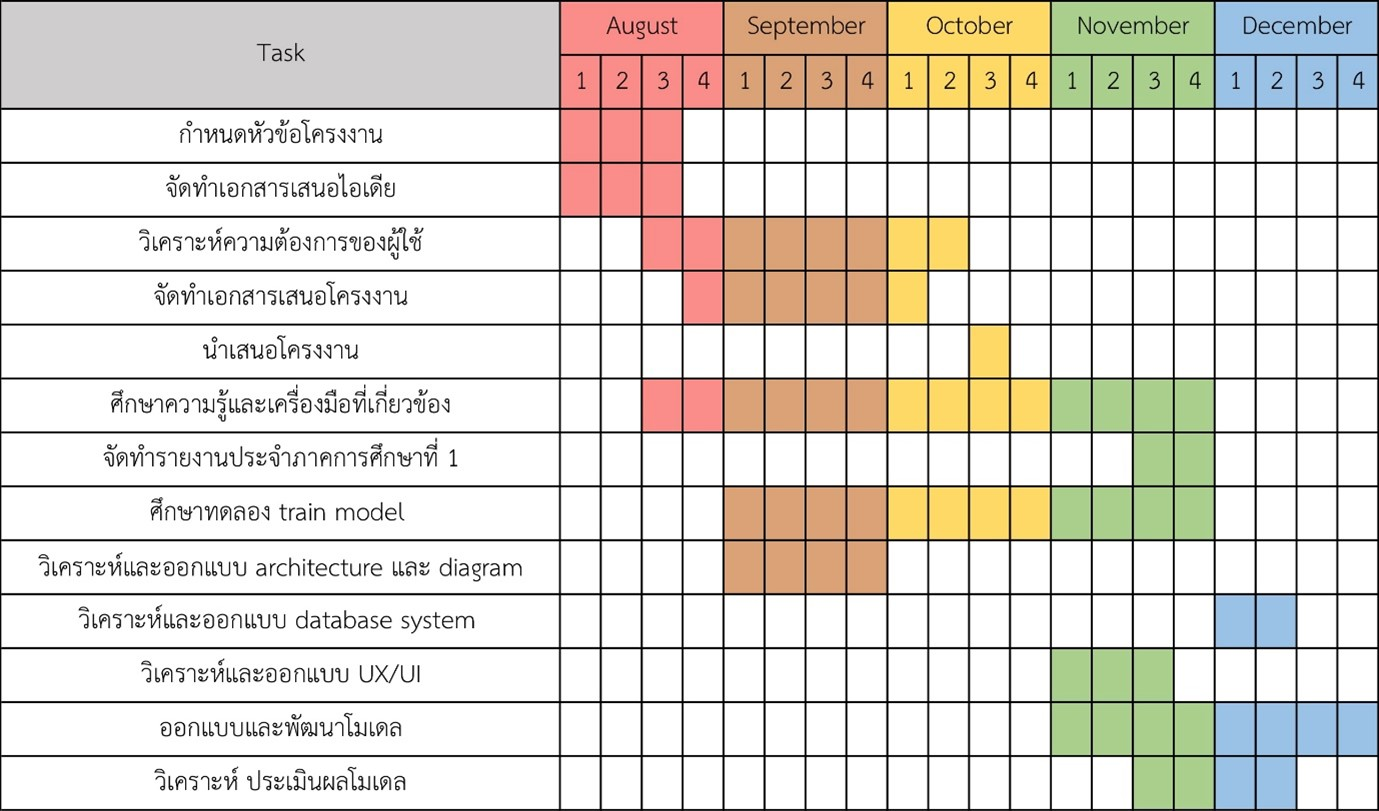
\includegraphics[width=13.8cm]{image/gantt-chart.jpg}
\caption{แสดงถึงแผนภูมิแกนต์ในการวางแผนงานในภาคเรียนที่ 1}
\label{fig:gantt-chart}
\end{figure}

\begin{figure}[!h]\centering
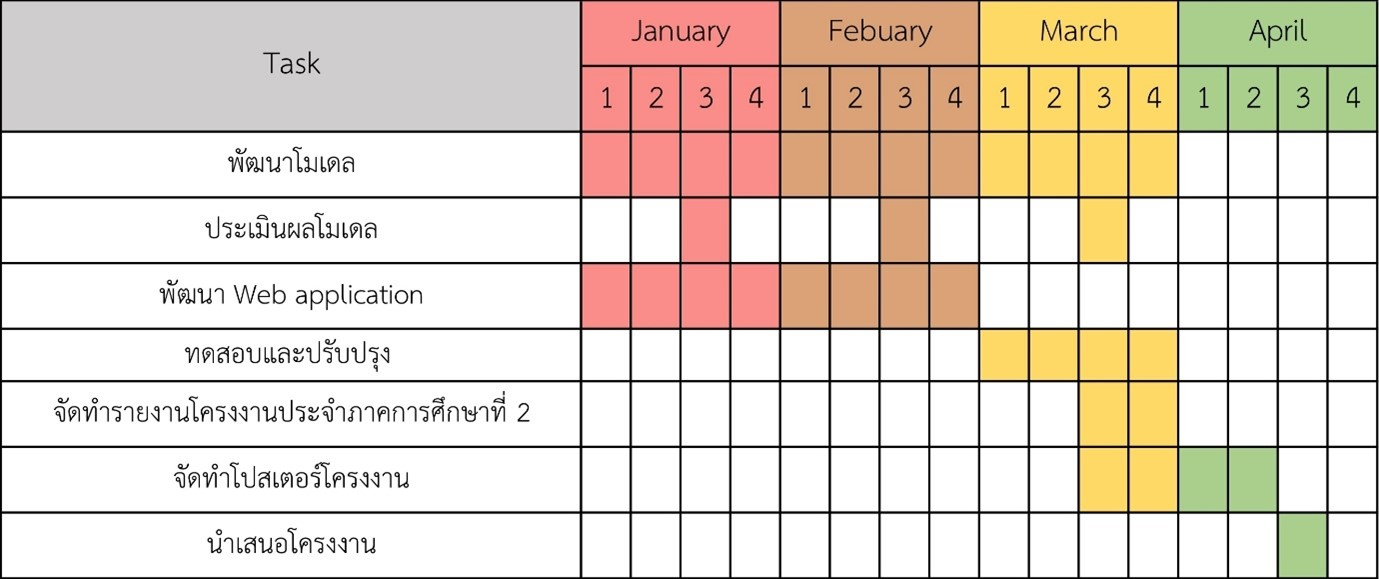
\includegraphics[width=13.8cm]{image/gantt-chart-2.jpg}
\caption{แสดงถึงแผนภูมิแกนต์ในการวางแผนงานในภาคเรียนที่ 2}
\label{fig:gantt-chart}
\end{figure}

\subsection{งานที่ได้รับผิดชอบของแต่ละบุคคล}

\hspace {18pt} ทางผู้จัดทำได้มีการแบ่งงานออกเป็น 3 ส่วนใหญ่ๆ คือ Front-End Back-End และ AI โดยจะแบ่งคนในกลุ่มรับผิดชอบงานแต่ละอันเป็นหลัก โดย

\begin{itemize}
\item นายพฤฒิพล จิตรเจริญกิจ รับผิดชอบในส่วนของ AI
\item นายวิชยุฒม์ ช่วยชูกูล รับผิดชอบในส่วนของ Front-End 
\item นายธัญพิสิษฐ์ พิสิฐพล รับผิดชอบในส่วนของ Back-End 
\end{itemize}

โดยหากงานในส่วนใดติดขัดสามารถให้ผู้จัดทำคนอื่นที่รับผิดชอบในส่วนอื่นมาช่วยแก้ไขปัญหาเพื่อให้งานมีความคืบหน้าไปอย่างรวดเร็ว

\subsection{ผลลัพธ์ที่คาดหวัง}

\begin{enumerate}
\item ภาพห้องที่ได้รับจากโมเดลที่ผ่านการ Train มีความเสมือนจริงและมีผลิตภัณฑ์จากฐานข้อมูลในเว็บไซต์เท่านั้น ภาพมีความละเอียด 1024 * 1024 Pixels และสามารถประเมินราคาเบื้องต้นของห้อง สามารถระบุจำนวนและเฟอร์นิเจอร์ที่ใช้พร้อมทั้งรายละเอียดทั้งหมดคือ ราคา สถานที่จำหน่าย ขนาด  
\item สามารถตรวจจับเฟอร์นิเจอร์ต่างๆที่อยู่ในรูปภาพและสามารถระบุจำนวนและเฟอร์นิเจอร์ที่ใช้พร้อมทั้งรายละเอียดทั้งหมดคือ ราคา สถานที่จำหน่าย ขนาด   
\item Web Application สามารถใช้งานโมเดลในการออกแบบภายใน 
\end{enumerate}

\subsection{ผลการดำเนินงานในภาคการศึกษาที่ 1}

\begin{itemize}
\item ทดลองใช้งานและ Train โมเดลเบื้องต้นเพื่อเป็นแนวทางสำหรับการออกแบบและพัฒนาโมเดล
\item ศึกษาความรู้และเครื่องมือที่เกี่ยวข้องทั้งการพัฒนาเว็บแอปพลิเคชันและการพัฒนาโมเดล
\item วิเคราะห์ความต้องการของผู้ใช้
\item วิเคราะห์และออกแบบ UX/UI
\item วิเคราะห์และออกแบบ Database System
\item ออกแบบและพัฒนาโมเดล
\item วิเคราะห์และออกแบบ Architecture และ Diagram
\item จัดทำเอกสารและนำเสนอ
\end{itemize}

\subsection{ผลการดำเนินงานในภาคการศึกษาที่ 2}

\begin{itemize}
\item ทดสอบและปรับปรุงทั้ง Web Application และ โมเดล
\item จัดทำรายงาน โปสเตอร์และนำเสนอ
\item Web Application มีความสามารถตรงตามความต้องการของผู้ใช้งาน
\item โมเดลมีประสิทธิภาพในการสร้างรูปภาพที่สมเหตุสมผลตามเงื่อนไขที่ผู้ใช้งานระบุและสามารถตรวจจับรูปภาพเพื่อหาผลิตภัณฑ์ที่มีความใกล้เคียงกับผลิตภัณฑ์ในรูปภาพ
\end{itemize}

\chapter{ทฤษฎีและงานวิจัยที่เกี่ยวข้อง}

\section{บทนำ}
\hspace {18pt} ในส่วนบทที่ 2 จะกล่าวถึง แนวคิดและทฤษฎีที่เกี่ยวข้องที่ใช้ในการทำงานและการศึกษาเพื่อบรรลุวัตถุประสงค์ รวมถึงงานวิจัยที่เกี่ยวข้องที่ได้ใช้อ้างอิงเพื่อใช้เป็นแนวทางในการดำเนินการทำโครงงาน

\section{ทฤษฎีที่เกี่ยวข้อง}

\subsection{Diffusion Model}
\hspace {18pt}Diffusion Model [4] คือ Generative Model ซึ่งอยู่ในหมวดของ Unsupervised Learning
หลักการทำงานของ Diffusion Model นั้นคือการสร้างชุดข้อมูลขึ้นมาใหม่ จากชุดข้อมูลที่เคยผ่านการเรียนรู้มาแล้ว Diffusion Model มีกระบวนการหลักๆอยู่ 2 ขั้นตอนคือ

\subsubsection{Forward Diffusion}
\hspace {18pt} Forward Diffusion [8] เป็นกระบวนการเพิ่ม Gaussian Noise ให้กับรูปภาพ โดยจะเพิ่ม Gaussian Noise ไปเรื่อย ๆ จนกระทั่งรูปภาพหมดความเป็นรูปภาพและกลายเป็น Gaussian Noise ทั้งรูปภาพในที่สุด ดังภาพ~\ref{fig:forward}

\begin{figure}[!h]\centering
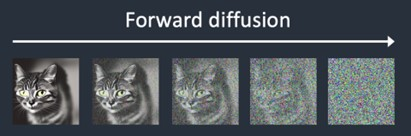
\includegraphics[width=10cm]{image/forward.jpg}
\caption{ตัวอย่างการทำงาน Forward Diffusion จาก \url{https://stable-diffusion-art.com/how-stable-diffusion-work/}}
\label{fig:forward}
\end{figure}

\subsubsection{Reverse Diffusion}
\hspace {18pt} Reverse Diffusion [9] เป็นกระบวนการกู้คืนรายละเอียดของรูปภาพ จากรูปภาพที่มี Gaussian Noise ให้กลับมามีรายละเอียดของรูปภาพเหมือนเดิมดังภาพ ~\ref{fig:reverse}

\begin{figure}[!h]\centering
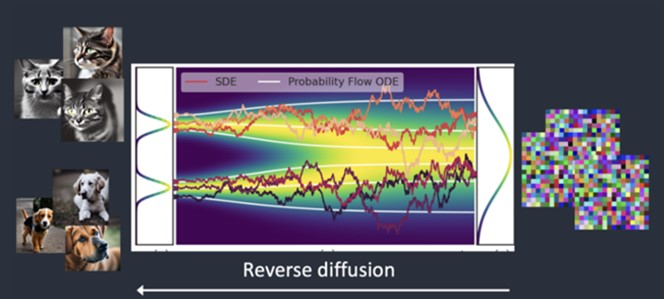
\includegraphics[width=10cm]{image/reverse.jpg}
\caption{ตัวอย่างการทำงาน Reverse Diffusion จาก \url{https://stable-diffusion-art.com/how-stable-diffusion-work/}}
\label{fig:reverse}
\end{figure}

\subsection{Stable Diffusion Model}
\hspace {18pt} Stable Diffusion Model เป็น Generative AI ที่พัฒนาต่อยอดมาจากแนวคิด Diffusion Model ในการ Generate รูปภาพออกมา วัตถุประสงค์เพื่อแก้ไขความล่าช้าอันเกิดมาจากขนาดของข้อมูลรูปภาพที่มีขนาดใหญ่และทำให้บริโภค GPU อย่างมากด้วยการใช้เทคนิคที่ชื่อว่า Variational Autoencoder

\begin{itemize}

\item \textbf {Variational Autoencoder (VAE)}
เป็น Convolutional Neural Network ที่ใช้ในการบีบอัด Dimensions ของข้อมูลลงเพื่อให้มีขนาดของข้อมูลที่เล็กลง สามารถลดลงไปได้ถึง 48 เท่าของขนาดภาพเดิม VAE ประกอบไปด้วย 2 ส่วนได้แก่

\begin{enumerate}
\item Encoder ทำหน้าที่บีบอัดข้อมูลให้กลายเป็น Latent Vector โดยจะกลายเป็น 4  Channel Grayscale  
\item Decoder ทำหน้าที่คลายขนาดข้อมูลจาก Latent Vector กลับไปเป็น รูปภาพตามเดิม 
\item Web Application สามารถใช้งานโมเดลในการออกแบบภายใน 
\end{enumerate}

Stable Diffusion Model จะทำการ Encode รูปภาพก่อนที่จะสู่กระบวนการทำ Forward Diffusion และหลังจากจบกระบวนการ Reverse Diffusion จะทำการ Decode Latent Vector ให้กลับมาเป็นรูปภาพปกติ ดังภาพ ~\ref{fig:autoencoder}

\begin{figure}[!h]\centering
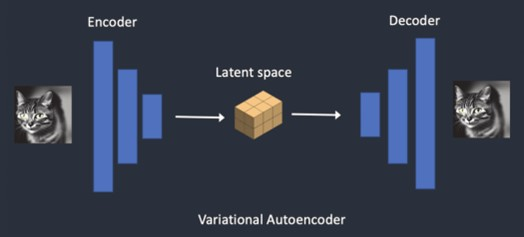
\includegraphics[width=10cm]{image/autoencoder.jpg}
\caption{ตัวอย่างการทำงาน Variational Autoencoder จาก \url{https://stable-diffusion-art.com/how-stable-diffusion-work/}}
\label{fig:autoencoder}
\end{figure}

กระบวนการทำงานของ Stable Diffusion Model ยังคงเหมือน  Diffusion Model แต่จะเพิ่มเติมการทำงานขึ้นมาดังนี้

\begin{enumerate}
\item Forward Diffusion ในระหว่างที่เพิ่ม Gaussian Noise ไปเรื่อย ๆ ในแต่ละรอบจะมีการ Training Noise Predictor 
(U-Net) [10] ให้จดจำจำนวนรอบที่เพิ่ม Gaussian Noise เข้าไป 
\item Reverse Diffusion ในขั้นตอนการ Reverse Diffusion ถ้าไม่มีการควบคุมให้กับกระบวนการนี้ผลลัพธ์ที่ได้จะไม่ต่างอะไรกับการสุ่มภาพออกมาเราจึงจำเป็นต้องมีการควบคุมเพื่อให้ได้ผลลัพธ์ที่เราต้องการ
\end{enumerate}

ในกรณีนี้คณะผู้จัดทำควบคุมด้วยข้อความคือการรับค่าเป็นข้อความแล้วได้ผลลัพธ์เป็นรูปภาพ โดยการที่รับข้อความแล้วออกมาเป็นรูปภาพ กลไกที่เป็นตัวควบคุมการย้อนกลับนั้นคือ Noise Predictor (U-Net) และ Scheduler ในการรับเงื่อนไขแล้วทำการลบ Gaussian Noise เรื่อยๆ จนได้ภาพที่ต้องการ กลไกตรงส่วนนี้จะเรียกว่าการทำ Denoising U-Net ดังภาพ~\ref{fig:u-net}

%%%%%%%%%%%%%%%%% Move to the next page %%%%%%%%%%%%%%%%
\vspace{\fill}\clearpage

\begin{figure}\centering
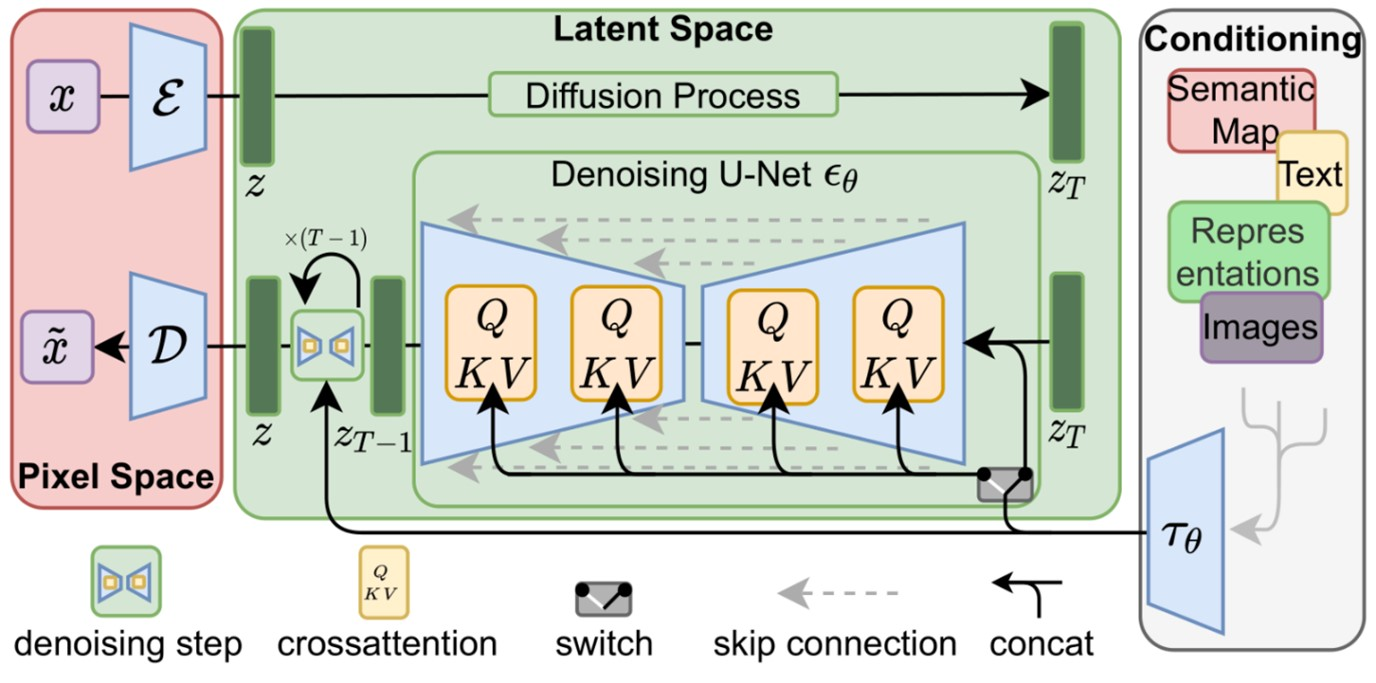
\includegraphics{image/u-net.jpg}
\caption{แสดงโครงสร้างของ Stable Diffusion จาก \url{https://arxiv.org/pdf/2112.10752.pdf}}
\label{fig:u-net}
\end{figure}

ในการรับข้อความแล้วได้ผลลัพธ์เป็นรูปภาพนั้นจะต้องทำการ Encode ข้อความด้วย Text Encoder ก่อนเพื่อให้กระบวนการ Denoising เข้าใจว่าความหมายของข้อความ (ให้ Machine เข้าใจภาษามนุษย์) ใน Stable Diffusion Model ใช้ CLIP ViT-L/14 [11]

\item \textbf{CLIP ViT-L/14}  Constrastive Language – Image Pre-training (CLIP) เป็น Neural Network Model ที่ทาง OpenAI พัฒนาขึ้น ด้วยการ Train ชุดข้อมูลการจับคู่ระหว่างรูปภาพและข้อความ เป็นจำนวน 400 ล้านคู่ มีความสามารถในการระบุข้อความและรูปภาพที่มีความหมายใกล้เคียงกันได้ ดังภาพ~\ref{fig:table-vector}

\begin{figure}[!h]\centering
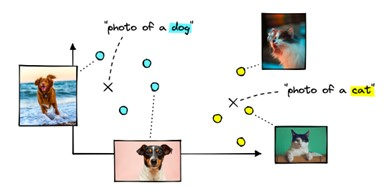
\includegraphics[width=8cm]{image/table-vector.jpg}
\caption{การจัดหมวดหมู่ตามความหมายของรูปภาพและข้อความของ CLIP ใน Table Vector เดียวกัน จาก \url{https://www.pinecone.io/learn/series/image-search/zero-shot-object-detection-clip/}}
\label{fig:table-vector}
\end{figure}

ภายใน CLIP จะประกอบไปด้วย 2 ส่วนคือ 1. Text Encoder 2. Image Encoder 
CLIP มีหลากหลาย Version แต่ Version ที่ Stable Diffusion ใช้คือ CLIP ViT-L/14 เพราะมีความแม่นยำสูง โดยมีความแม่นยำที่ 75.4\% กับ Imagenet top 1 ดังภาพ~\ref{fig:clip-vit}

%%%%%%%%%%%%%%%%% Move to the next page %%%%%%%%%%%%%%%%
\vspace{\fill}\clearpage

\begin{figure}[!h]\centering
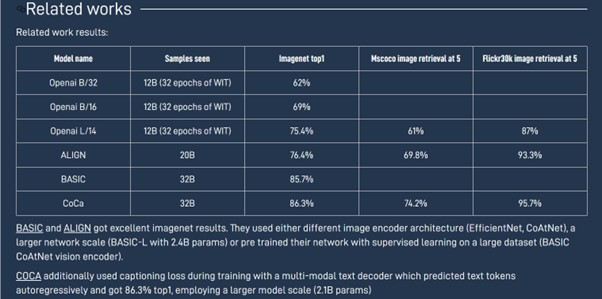
\includegraphics[width=11cm]{image/clip-vit.jpg}
\caption{แสดงถึงประสิทธิภาพของ CLIP ViT-L/14 (Openai L/14) เมื่อเทียบกับโมเดลอื่นๆ จาก \url{https://www.pinecone.io/learn/series/image-search/zero-shot-object-detection-clip/}}
\label{fig:clip-vit}
\end{figure}

\item \textbf{Denoising U-net}
U-net [10] เป็น Convolutional Neural Network ที่ใช้ในงาน Computer Vision ในที่นี้ U-net มีหน้าที่รับข้อความที่ผ่านการ Encode มาแล้วจาก CLIP Text Encoder ข้อความที่ผ่านการ Encode มาแล้วจะเป็นเงื่อนไขที่คอยบังคับทิศทางให้กับ U-Net ในขั้นตอนการ Denoising เพื่อให้ได้รูปภาพสอดคล้องกับข้อความมากที่สุด
\end{itemize}

\subsection{LoRA model}
\hspace {18pt} มีโมเดลอยู่ไม่น้อยที่มีขนาดที่ใหญ่ขึ้นและมีความซับซ้อนที่มากขึ้น ทำให้การ Train โมเดลใหม่หรือ การ Fine-Tuning โมเดล ต้องใช้เวลาที่นานขึ้นและทรัพยากรที่มากขึ้นตามไปด้วย 

\hspace {18pt} Low-Rank Adaptation (LoRA) [6] ในภาพ~\ref{fig:lora} เป็นเทคนิคการทำ Fine-Tuning ให้กับโมเดล Diffusion Model โดยใช้โมเดลที่ Pre-trained มาเป็น weight initialize และจะทำการ Freeze layer ของ Pre-trained และ Train เพิ่มแค่ในส่วนของ Weight ใหม่ เข้าไปให้กับ Model ใหม่ ข้อดีคือสามารถลดจำนวน parameter ที่ใช้ ได้ถึง 10000 เท่าและลดปริมาณการบริโภค GPU ถึง 3 เท่าเมื่อเปรียบเทียบกับโมเดล GPT-3 175B Fine-Tuned with Adam [7] 

\begin{figure}[!h]\centering
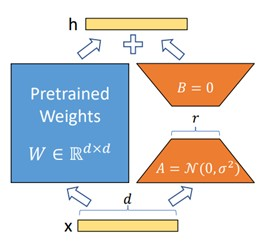
\includegraphics[width=7cm]{image/lora.jpg}
\caption{แสดงโครงสร้างการทำงานของ LoRA จาก \url{https://arxiv.org/pdf/2106.09685.pdf}}
\label{fig:lora}
\end{figure}

%%%%%%%%%%%%%%%%% Move to the next page %%%%%%%%%%%%%%%%
\vspace{\fill}\clearpage

\subsection{Dreambooth}
\hspace {18pt} ในขณะที่ text-to-image โมเดลเป็นการก้าวกระโดดไปอีกขั้นของ AI ทั้งมีคุณภาพที่ดี และยัง Generate รูปภาพได้จากการให้ใส่ข้อความบางอย่างลงไป [12] ปัญหาคือถ้าต้องการให้โมเดลสามารถเรียนรู้บางสิ่งบางอย่างที่เฉพาะเจาะจงมากยิ่งขึ้น จะสามารถ Training ได้อย่างไร

\hspace {18pt} Dreambooth [13] เป็น Personalization text-to-image  โมเดล พัฒนาโดย Google Research Team เพื่อให้ Diffusion Model สามารถที่จะรู้จักวัตถุที่มีความเฉพาะเจอะจงมากขึ้นได้ สามารถ Training ภาพและข้อความที่จับคู่กับรูปภาพเพิ่มเติมเข้าไปเพื่อให้โมเดลสามารถเรียนรู้ได้เฉพาะเจาะจงมากยิ่งขึ้น ให้ตรงตามเป้าหมายของผู้ใช้มากขึ้น

\subsection{Object Detection}
\hspace {18pt}Object Detection [26]  เป็นงานของ Computer Vision มีเป้าหมายเพื่อทำการตรวจจับวัตถุต่าง ๆ ที่สนใจ และจำแนกออกไปตามหมวดหมู่ต่าง ๆ ที่ได้กำหนดไว้ ตัวอย่างการใช้งาน เช่น การตรวจจับใบหน้าของคน การตรวจจับคนบนทางเท้า การตรวจจับรถยนต์ด้วยกล้องวงจรปิด

\subsection{Zero-shot Object Detection}
\hspace {18pt} Zero-shot [27] เป็นเทคนิคการใช้งานโมเดลที่ผ่านการ training มาแล้วด้วยชุดข้อมูล Domain หนึ่ง และนำมาใช้ในการทำนายในอีกชุดข้อมูลที่ Domain ไม่ได้ผ่านการเรียนรู้มาก่อน

\hspace {18pt}Zero-shot Object Detection with CLIP เป็นการนำโมเดล CLIP ของ OpenAI มาใช้ในการทำ Object Detection รูปภาพโดยที่จะรับรูปภาพและข้อความที่จะใช้ในการจำแนกว่ารูปว่ามีความหมายตรงกับข้อความใด ดังภาพ~\ref{fig:zero-shot}


\begin{figure}[!h]\centering
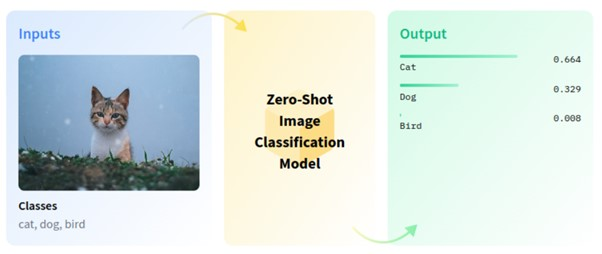
\includegraphics[width=9cm]{image/zero-shot.jpg}
\caption{แสดงการทำงานของ Zero-Shot Image Classification โดยใช้โมเดล CLIP ของ OpenAI จาก \url{https://docs.openvino.ai/2022.3/notebooks/228-clip-zero-shot-image-classification-with-output.html}}
\label{fig:zero-shot}
\end{figure}

แต่ข้อจำกัดของโมเดล CLIP คือไม่สามารถตรวจจับได้หลายวัตถุ การที่จะทำให้โมเดล CLIP สามารถตรวจจับวัตถุได้มากกว่า 1 วัตถุนั้นจะต้องทำการแบ่งรูปภาพออกเป็นส่วน ๆ และทำการตรวจจับภาพทีละส่วนแทน 
ดังภาพ~\ref{fig:zero-shot-model} จึงทำให้ CLIP สามารถตรวจจับได้หลายวัตถุได้

\begin{figure}[!h]\centering
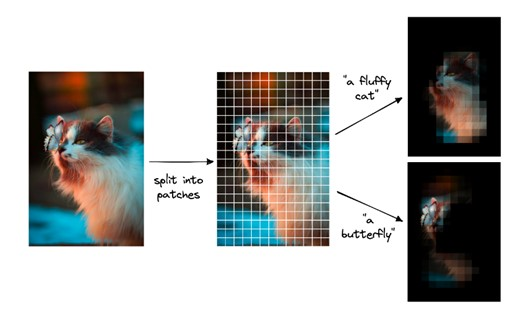
\includegraphics[width=8cm]{image/zero-shot-model.jpg}
\caption{แสดงการตรวจจับด้วยโมเดลในส่วนต่างๆขอองรูปภาพที่ถูกแบ่ง จาก \url{https://www.pinecone.io/learn/series/image-search/zero-shot-object-detection-clip/}}
\label{fig:zero-shot-model}
\end{figure}

\section{งานวิจัยที่เกี่ยวข้อง}

\subsection{Stable Diffusion}
\hspace {18pt}Stable Diffusion [4] เปิดตัวโดย StabilityAI ในปี 2022 เป็น Generative AI ที่สามารถทำได้หลายอย่างทั้ง text-to-image หรือคือการสร้างรูปภาพจากข้อความ (Prompt) Image-to-Image หรือการสร้างรูปภาพจากรูปภาพ in-painting ซึ่งคือการปรับแต่งรูปภาพเช่น การเพิ่มวัตถุ การลบวัตถุออกจากภาพ นอกจากนี้โค้ดของโมเดลยังสามารถเข้าถึงได้ฟรี สามารถปรับแต่งโมเดลได้ มี Community ที่หนาแน่น เช่น Civit.ai ที่มีโมเดล Stable Diffusion ที่ปรับแต่งให้เข้ากับการสร้างรูปภาพในหลากหลายสไตล์ สามารถใช้ในคอมพิวเตอร์ที่ใช้ Windows MacOS หรือ Linux มี RAM อย่างน้อย 16 GB มี Nvidia GPU ที่มี VRAM อย่างน้อย 10 GB มีพื้นที่ว่างอย่างน้อย 12 GB [14]

\hspace {18pt} จากงานวิจัยจากแหล่งภายนอก ทางคณะผู้จัดทำพบว่า Stable Diffusion มีคะแนน FID [15] ที่ต่ำกว่า Midjourney จากการสร้างรูปภาพใบหน้าคน 5,000 รูป และคำนวณ FID scores โดยทำขั้นตอนนี้เป็นจำนวน 10 ครั้ง จากนั้นคำนวณค่าเฉลี่ยและส่วนเบี่ยงเบนมาตรฐานของ FID คะแนน FID ดังภาพ~\ref{fig:fid} Stable Diffusion ให้คะแนน FID ที่ต่ำกว่า ดังนั้นจึงสร้างรูปใบหน้าคนได้ใกล้เคียงรูปจริงมากกว่า Midjourney

\begin{figure}[!h]\centering
\fbox{\includegraphics[width=9cm]{image/fid.jpg}}
\caption{ภาพคะแนน FID ของโมเดล จากการสุ่มชุดข้อมูล 5,000 รูป จาก \url{https://arxiv.org/pdf/2210.00586.pdf}}
\label{fig:fid}
\end{figure}

\subsection{เว็บแอปพลิเคชัน Interior AI}
\hspace {18pt} เว็บแอปพลิเคชัน Interior AI[17] เป็นเว็บแอปพลิเคชันที่ใช้ในการออกแบบภายใน โดยจะรับข้อมูลเป็นรูปภาพของห้อง เลือกชนิดของห้องได้กว่า 30 ชนิด เลือกสไตล์ของห้องได้กว่า 35 สไตล์ เลือกความละเอียดของรูปภาพ เลือกโหมดที่ต้องการ ซึ่งจะมีให้เลือกดังนี้ Interior Design Freestyle Virtual Staging และ 360 panorama เลือกความเป็นส่วนตัวของรูป หากเลือกให้เป็น Public จะเผยแพร่ไปที่หน้าเว็บซึ่งจะแสดงภาพต่างๆที่ถูก Generate ล่าสุด ดังภาพ~\ref{fig:interior-ai-2} และสามารถค้นหาเฟอร์นิเจอร์ที่ใช้ในรูปภาพได้ด้วย Google Lens โดยผลลัพธ์ที่ได้จะเป็นรูปภาพที่คล้ายกัน ไม่สามารถบ่งบอกแหล่งจัดซื้อเฟอร์นิเจอร์ได้ ไม่มีรายละเอียดข้อมูลของเฟอร์นิเจอร์ดังภาพ~\ref{fig:interior-ai} รวมถึงมีระบบสมัครสมาชิกซึ่งจำเป็นจะต้องเป็นสมาชิกก่อนถึงจะใช้งาน AI ได้ 

%%%%%%%%%%%%%%%%% Move to the next page %%%%%%%%%%%%%%%%
\vspace{\fill}\clearpage

\begin{figure}[!h]\centering
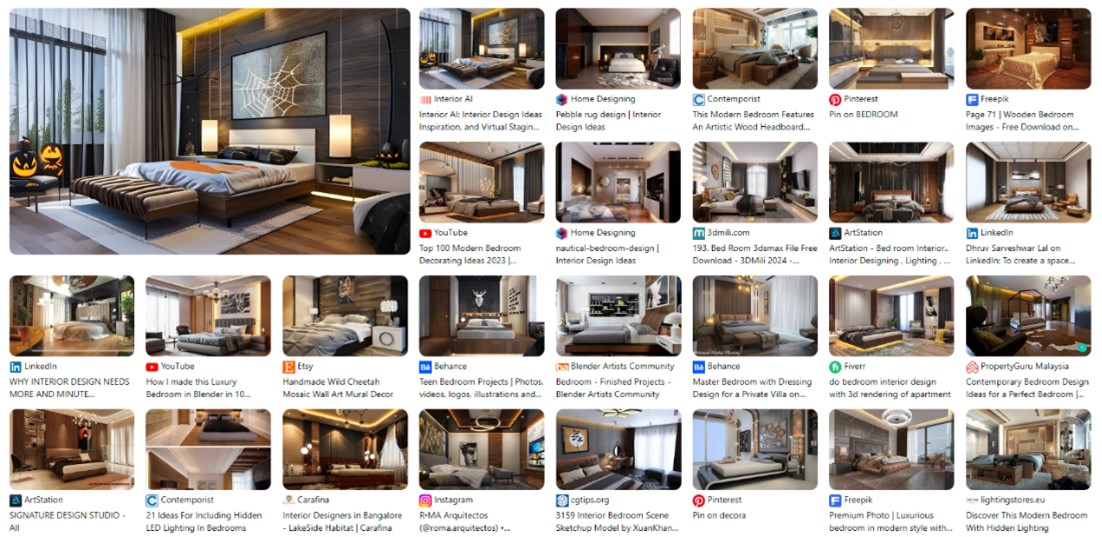
\includegraphics[width=9cm]{image/interior-ai.jpg}
\caption{ตัวอย่างการค้นหาเฟอร์นิเจอร์จากรูปภาพด้วย Google Lens ในเว็บแอปพลิเคชัน Interior AI จาก \url{https://interiorai.com/}}
\label{fig:interior-ai}
\end{figure}

\begin{figure}[!h]\centering
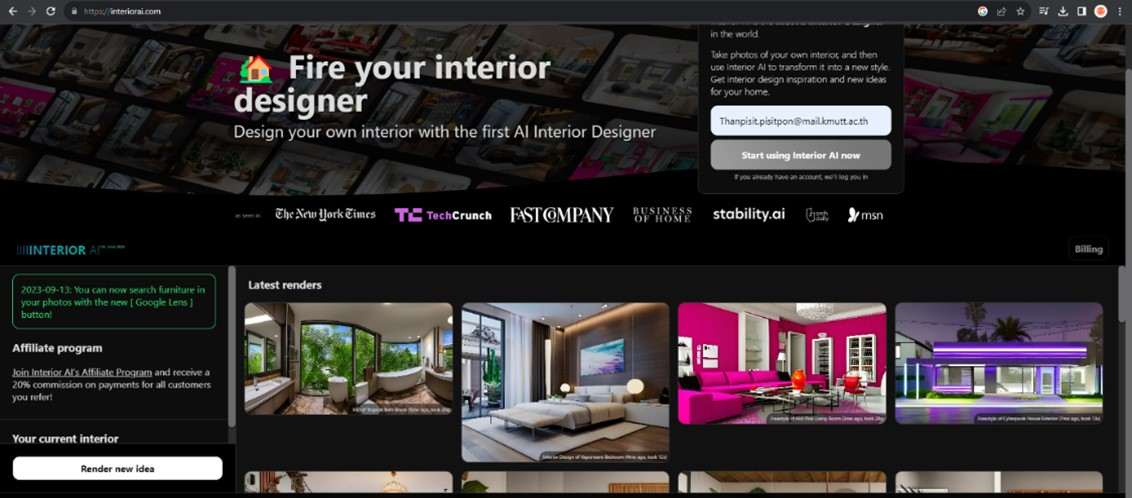
\includegraphics[width=9cm]{image/interior-ai-2.jpg}
\caption{ตัวอย่างหน้าหลักของเว็บแอปพลิเคชัน Interior AI ที่มีแบ่งปันไอเดียการออกแบบภายในจากภาพที่ จาก \url{https://interiorai.com/}}
\label{fig:interior-ai-2}
\end{figure}

\begin{table}[!h]
\caption{ตารางเปรียบเทียบเว็บแอปพลิเคชันของคณะผู้จัดทำกับ เว็บแอปพลิเคชัน Interior AI }\label{tbl:interior-ai-table}
  \begin{tabular}{|p{4cm}|p{5cm}|p{5cm}|}
  \hline
  \textbf{Features} & \textbf{ Interior AI} & \textbf{Easy room } \\
  \hline
  เข้าสู่ระบบ / ออกจากระบบ & ไม่สามารถออกจากระบบ & สามารถทำได้ทั้งหมด \\
  \hline
  ลงทะเบียน & มี & มี \\
  \hline
  สร้างรูปภาพ & ต้องเป็นสมาชิกถึงจะใช้งานได้ใช้รูปภาพระบุชนิดและสไตล์ของห้องเป็นอินพุตโหมดการrenderเลือกResolutionผลลัพธ์ที่ได้คือภาพ 1 รูป มีชนิดและสไตล์ของห้องที่หลากหลายสร้างpanoramaได้ & ระบุชนิดและสไตล์ของห้องผลิตภัณฑ์ที่ใช้และระบุงบประมาณโดยรวมผลลัพธ์ที่ได้คือภาพ 1 รูป พร้อมมูลค่าโดยรวมของเฟอร์นิเจอร์ที่ใช้แหล่งจำหน่ายเฟอร์นิเจอร์ \\
  \hline
  ตรวจจับผลิตภัณฑ์ & มี & มี \\
  \hline
  ประวัติการใช้งาน & ไม่มี & มี \\
  \hline
  แบ่งปันไอเดีย & มี แต่สามารถเลือกได้ว่าจะแบ่งปันหรือไม่ & มี แต่สามารถเลือกได้ว่าจะแบ่งปันหรือไม่ \\
  \hline
  ประวัติการใช้งาน & ไม่มี & ไม่มี \\
  \hline
\end{tabular}
\end{table}

\subsection{เว็บแอปพลิเคชัน AI ROOM PLANNER}
\hspace {18pt} เว็บแอปพลิเคชัน AI ROOM PLANNER [18] เป็นเว็บแอปพลิเคชันที่ใช้สำหรับปรับเปลี่ยนดีไซน์ของห้อง โดยจะรับอินพุตเป็น รูปภาพของห้อง เลือกชนิดของห้องได้กว่า 25 ชนิด เลือกสไตล์ห้องได้กว่า 32 สไตล์  ไม่มีระบบสมาชิก ใช้งานได้ฟรี โดยตัวอย่างการใช้งาน AI เว็บไซต์จะเป็นดังภาพ~\ref{fig:planner}

\begin{figure}[!h]\centering
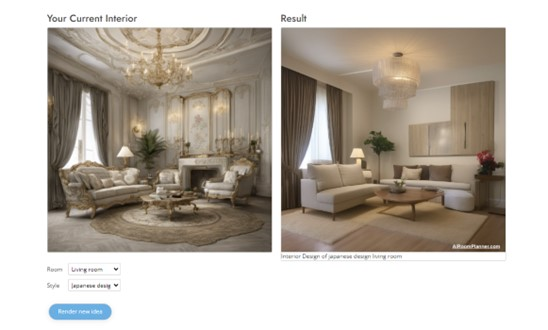
\includegraphics[width=9cm]{image/planner.jpg}
\caption{ตัวอย่างการใช้งาน AI ในเว็บแอปพลิเคชัน AI ROOM PLANNERทางซ้ายของภาพเป็นภาพต้นแบบที่ทำการอินพุตและภาพทางขวาคือภาพที่ AI สร้างขึ้น จาก \url{https://airoomplanner.com/}}
\label{fig:planner}
\end{figure}

\begin{table}[!h]
\caption{ตารางเปรียบเทียบเว็บแอปพลิเคชันของคณะผู้จัดทำกับ เว็บแอปพลิเคชัน Ai Room Planner }\label{tbl:planner-table}
  \begin{tabular}{|p{4cm}|p{5cm}|p{5cm}|}
  \hline
  \textbf{Features} & \textbf{AI ROOM PLANNER} & \textbf{Easy room } \\
  \hline
  เข้าสู่ระบบ / ออกจากระบบ & ไม่สามารถออกจากระบบ & สามารถทำได้ทั้งหมด \\
  \hline
  ลงทะเบียน & มี & มี \\
  \hline
  สร้างรูปภาพ & ใช้รูปภาพชนิดและสไตล์ของห้องเป็นอินพุต มีชนิดและสไตล์ของห้องที่หลากหลาย ผลลัพธ์ที่ได้คือ ภาพ 1 รูป  & ระบุชนิดและสไตล์ของห้องผลิตภัณฑ์ที่ใช้และระบุงบประมาณโดยรวม ผลลัพธ์ที่ได้คือ ภาพ 1 รูป พร้อมมูลค่าโดยรวมของเฟอร์นิเจอร์ที่ใช้ แหล่งจำหน่ายเฟอร์นิเจอร์ \\
  \hline
  ตรวจจับผลิตภัณฑ์ & ไม่มี & มี \\
  \hline
  ประวัติการใช้งาน & ไม่มี & มี \\
  \hline
  แบ่งปันไอเดีย & มี  & มี แต่สามารถเลือกได้ว่าจะแบ่งปันหรือไม่ \\
  \hline
  ประวัติการใช้งาน & ไม่มี & ไม่มี \\
  \hline
\end{tabular}
\end{table}

\subsection{เว็บแอปพลิเคชัน Spacely AI}
\hspace {18pt} เว็บแอปพลิเคชัน Spacely AI[19] เป็นเว็บแอปพลิเคชันที่ใช้ในการออกแบบภายใน มีคณะผู้จัดทำทั้งหมด 9 คน [29] มี target user เป็นดีไซนเนอร์ มีจุดประสงค์ที่จะทำเว็บแอปพลิเคชันคล้ายๆ Canva สำหรับดีไซน์เนอร์ เนื่องจากเครื่องมือในการออกแบบนั้นค่อนข้างแพงและยากที่จะใช้งาน [28]    มีฟีเจอร์ที่หลากหลายทั้ง การปรับเปลี่ยนสไตล์ของห้อง การลบสิ่งของในรูปภาพ การเปลี่ยนสิ่งของในรูปภาพ และสามารถค้นหาเฟอร์นิเจอร์ได้ดังภาพ~\ref{fig:spacely} มีระบบสมาชิก และสามารถใช้งานได้ฟรีในบางฟีเจอร์ สามารถเลือกได้ว่าจะแชร์รูปที่ได้จากการทำงานของ AI ได้ และสามารถสร้างห้องจาก Prompt ที่เป็นข้อความได้อีกด้วย 

\begin{figure}[!h]\centering
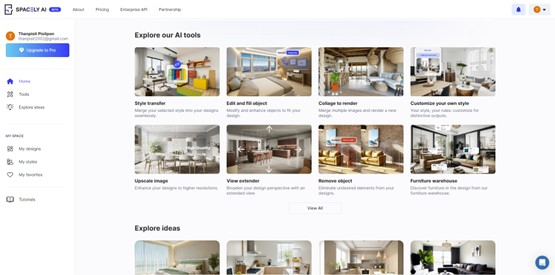
\includegraphics[width=9cm]{image/spacely.jpg}
\caption{แสดงความสามารถทั้งหมดของ Ai ในเว็บแอปพลิเคชัน spacely.ai จาก \url{https://www.spacely.ai/}}
\label{fig:spacely}
\end{figure}

%%%%%%%%%%%%%%%%% Move to the next page %%%%%%%%%%%%%%%%
\vspace{\fill}\clearpage

 ตัวอย่างฟีเจอร์ที่น่าสนใจของเว็บแอปพลิเคชัน Spacely AI คือ

\begin{enumerate}
\item การปรับเปลี่ยนสไตล์ของภาพห้อง   
\par \hspace {18pt} เว็บแอปพลิเคชัน Spacely AI สามารถปรับเปลี่ยนสไตล์ของห้องได้โดยจะรับอินพุตเป็น ภาพของห้องที่มีการปรับเปลี่ยนสไตล์และภาพของห้องที่มีสไตล์ที่อยากเปลี่ยนซึ่งผลลัพธ์จะเป็นดังภาพ~\ref{fig:spacely1-1} โดยภาพทางฝั่งซ้ายจะเป็นภาพของห้องที่ผู้ใช้ต้องการจะปรับเปลี่ยนสไตล์และภาพฝั่งขวาจะเป็นภาพที่ผ่านการปรับเปลี่ยนสไตล์จาก AI ของเว็บแอปพลิเคชัน Spacely AI

\begin{figure}[!h]\centering
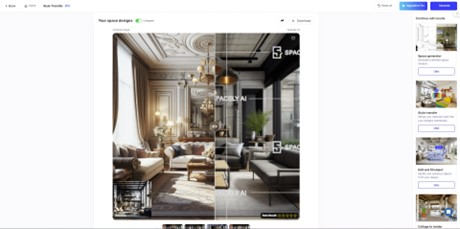
\includegraphics[width=9cm]{image/spacely1-1.jpg}
\caption{ผลลัพธ์จากฟีเจอร์การปรับเปลี่ยนสไตล์ห้องของเว็บแอปพลิเคชัน Spacely AI จาก \url{https://www.spacely.ai/}}
\label{fig:spacely1-1}
\end{figure}

\item การตรวจจับเฟอร์นิเจอร์ 
\par \hspace {18pt} เว็บแอปพลิชัน Spacely AI มีความสามารถในการตรวจจับเฟอร์นิเจอร์ภายในภาพโดยรับอินพุตเป็นภาพซึ่งผลลัพธ์ที่ได้นั้นจะเป็นเฟอร์นิเจอร์ที่มีความใกล้เคียงกับในภาพ มีการระบุมูลค่าของเฟอร์นิเจอร์ หาซื้อได้ผ่าน eBay Houzz AliExpress Amazon เป็นต้น ซึ่งมีความเป็นไปได้ว่าจะเป็นผลิตภัณฑ์ที่มีการลงทะเบียนเป็น partner กันและเป็นโมเดลที่สร้างขึ้นเอง ดังภาพ~\ref{fig:spacely1-2}

\begin{figure}[!h]\centering
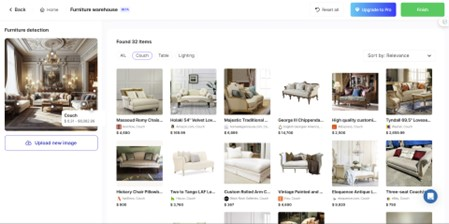
\includegraphics[width=9cm]{image/spacely1-2.jpg}
\caption{ผลลัพธ์จากฟีเจอร์การตรวจจับเฟอร์นิเจอร์ภายในภาพของเว็บแอปพลิเคชัน Spacely AI จาก \url{https://www.spacely.ai/}}
\label{fig:spacely1-2}
\end{figure}

\item การสร้างรูปภาพจากข้อความ (text to image)  
\par \hspace {18pt} เว็ปแอปพลิเคชัน Spacely AI สามารถสร้างรูปภาพข้อความโดยจะรับอินพุตเป็นข้อความซึ่งจะได้ผลลัพธ์เป็นรูปภาพ 4 ภาพทีแตกต่างกันหากต้องการที่จะทราบรายละเอียดเฟอร์นิเจอร์ที่ใช้จะต้องโหลดรูปภาพและนำไปใช้งานกับฟีเจอร์ตรวจจับเฟอร์นิเจอร์ มีตัวอย่างดังนี้ 
\par 
ข้อความที่อินพุต "Generate a highly realistic image of a minimal-style living room that resembles an authentic photograph. The room should embody the essence of minimalism with lifelike architectural details, realistic furnishings, a subdued color palette, and convincing lighting, shadows, and reflections. Make it appear as though you're looking at a real photograph of a minimal-style living room"
ผลลัพธ์ที่ได้จะเป็นดังภาพ~\ref{fig:spacely-gen}

%%%%%%%%%%%%%%%%% Move to the next page %%%%%%%%%%%%%%%%
\vspace{\fill}\clearpage

\begin{figure}[!h]\centering
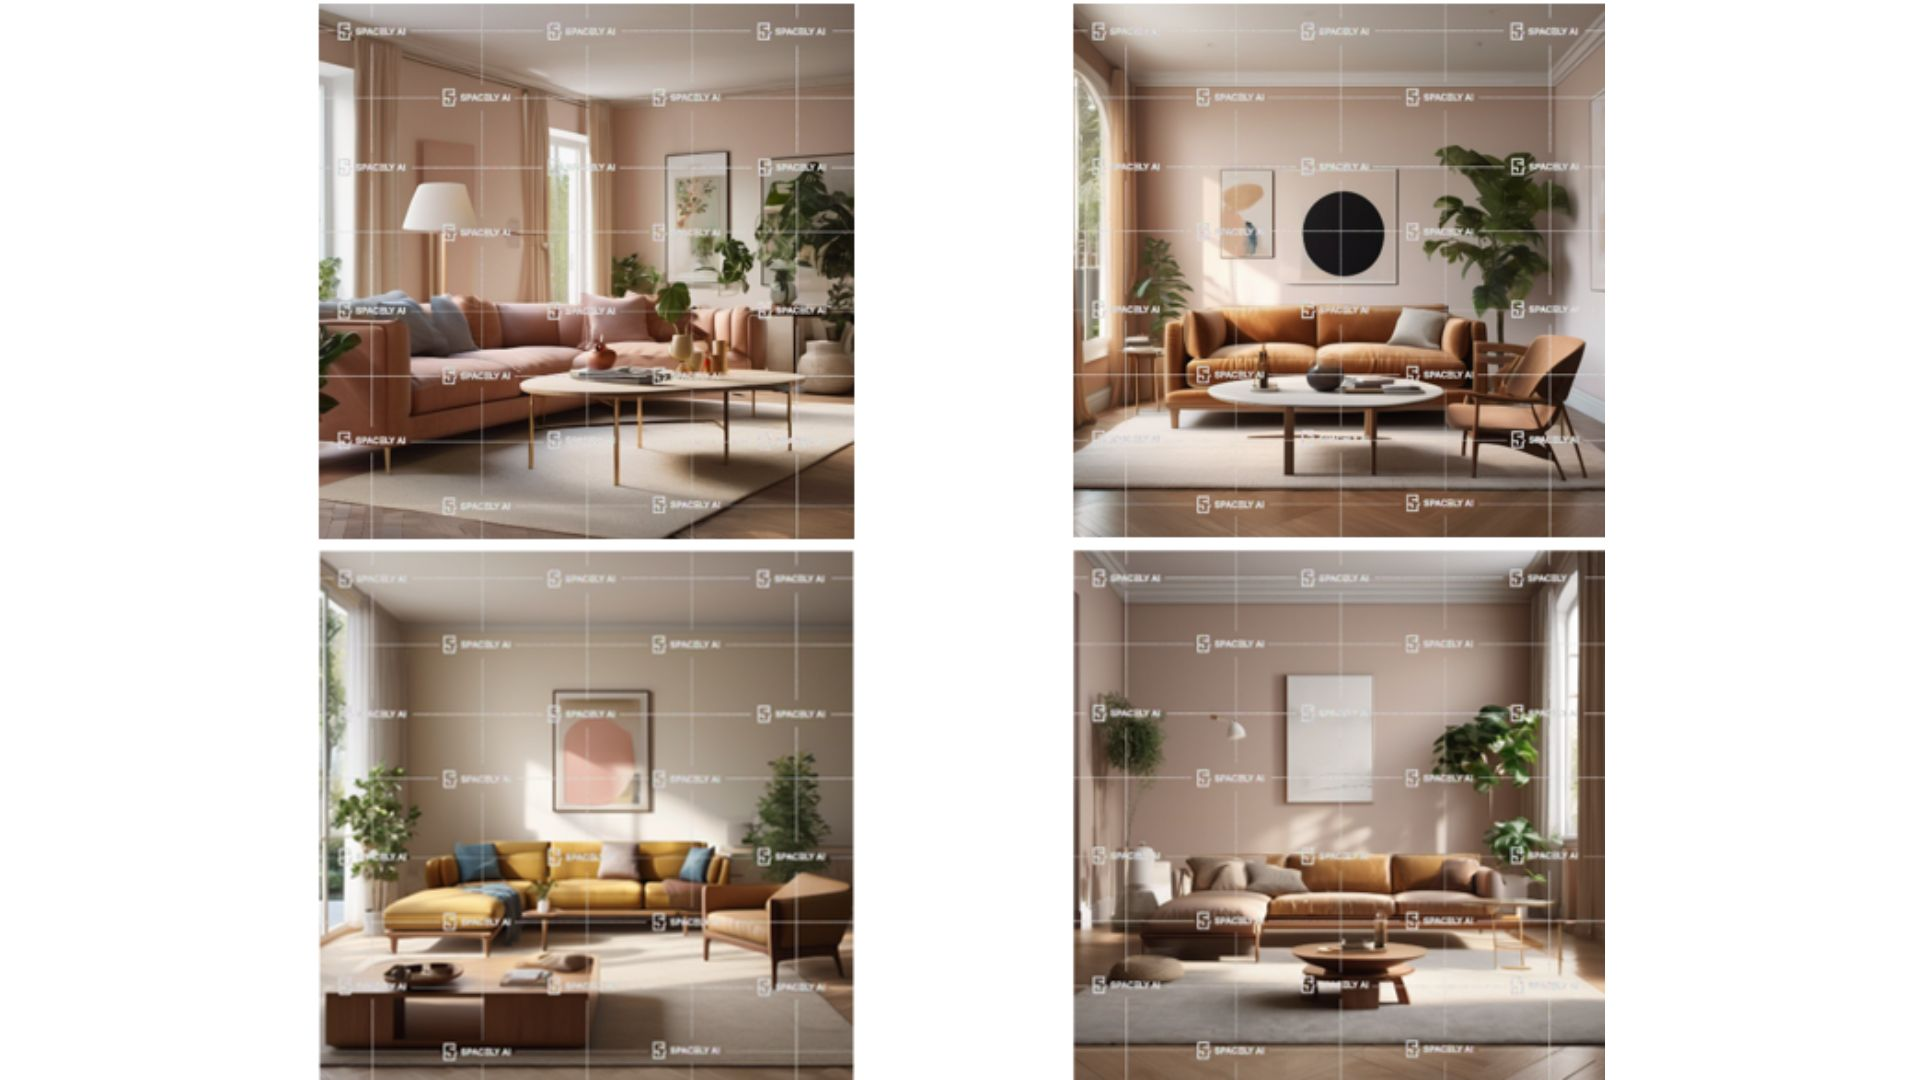
\includegraphics[width=10cm]{image/spacely-gen.jpg}
\caption{ผลลัพธ์ของการสร้างรูปภาพจากข้อความของเว็บแอปพลิเคชัน Spacely AI จาก \url{https://www.spacely.ai/}}
\label{fig:spacely-gen}
\end{figure}

\begin{table}[!h]
\caption{ตารางเปรียบเทียบเว็บแอปพลิเคชันของคณะผู้จัดทำกับ เว็บแอปพลิเคชัน Ai Room Planner }\label{tbl:planner-table}
  \begin{tabular}{|p{4cm}|p{5cm}|p{5cm}|}
  \hline
  \textbf{Features} & \textbf{Spacely AI} & \textbf{Easy room } \\
  \hline
  เข้าสู่ระบบ / ออกจากระบบ & สามารถทำได้ทั้งหมด & สามารถทำได้ทั้งหมด \\
  \hline
  ลงทะเบียน & มี & มี \\
  \hline
สร้างรูปภาพ & ไม่จำเป็นจะต้องเป็นสมาชิกก็สามารถใช้งานได้ แต่รูปที่ได้จะติดลายน้ำสามารถสร้างรูปภาพจากอินพุดที่เป็นข้อความเพียงอย่างเดียวได้
สามารถสร้างรูปภาพได้หลากหลายจุดประสงค์ เช่น ปรับเปลี่ยนสไตล์ของภาพเก่า เป็นต้น มีชนิดและสไตล์ของห้องที่หลากหลาย & ระบุชนิดและสไตล์ของห้อง ผลิตภัณฑ์ที่ใช้และระบุงบประมาณโดยรวม ผลลัพธ์ที่ได้คือ ภาพ 1 รูป พร้อมมูลค่าโดยรวมของเฟอร์นิเจอร์ที่ใช้ แหล่งจำหน่ายเฟอร์นิเจอร์ \\
  \hline
  ตรวจจับผลิตภัณฑ์ & มี & มี \\
  \hline
  ประวัติการใช้งาน & ไม่มี & มี \\
  \hline
  แบ่งปันไอเดีย & มี  & มี แต่สามารถเลือกได้ว่าจะแบ่งปันหรือไม่ \\
  \hline
  ประวัติการใช้งาน & มี & ไม่มี \\
  \hline
\end{tabular}
\end{table}

\end{enumerate}

%%%%%%%%%%%%%%%%% Move to the next page %%%%%%%%%%%%%%%%
\vspace{\fill}\clearpage

\section{เนื้อหาทางวิศวกรรมต้นฉบับ}

\subsection{แบบแผนการออกแบบโครงสร้างซอฟต์แวร์}
\hspace {18pt}ทางคณะผู้จัดทำได้เลือกใช้ Client-Server Model เป็นโมเดลโครงสร้างพื้นฐานสำหรับเว็บแอปพลิเคชัน เพราะเว็บแอปพลิเคชัน Easy Room สามารถเข้าใช้งานได้หลายคนในเวลาเดียวกัน Client-Server Model จึงเป็นโครงสร้างที่เหมาะสมในการนำมาใช้ [21] และเพื่อให้การพัฒนาซอฟต์แวร์นั้นทำได้ง่ายขึ้น [20] ทางคณะผู้จัดทำได้เลือก MVC Architecture เพื่อใช้ในการแยกส่วนการทำงานให้ออกมาเป็น 3 ส่วนด้วยกัน ได้แก่ 1. Model 2. View 3. Controller และเพื่อเพิ่มความปลอดภัยให้ได้มากที่สุดจึงได้มีการทำ Proxy Server มาเป็นตัวกลางการติดต่อระหว่าง Client และ Server [22, 23] และเนื่องจากเว็บแอปพลิเคชัน Easy Room มีการใช้ Stable diffusion ในส่วนของการ Generate รูปภาพขึ้นมาซึ่งมีความจำอย่างมากที่จะต้องใช้ GPU [14] ในการประมวล ณ ปัจจุบันเว็บแอปพลิเคชัน Easy Room ไม่สามารถใช้งาน GPU ได้หลายคนในเวลาเดียวกัน ทางคณะผู้จัดทำจึงเลือกที่จะทำ Load balance [24] เพื่อใช้ในการจัดการการเข้าใช้งาน GPU บนเว็บแอปพลิเคชัน Easy Room

\begin{itemize}
\item \textbf {Model View Controller (MVC Architecture)}
Model View Controller (MVC Architecture) [20] คือรูปแบบการออกแบบพัฒนาซอฟต์แวร์ ดังภาพ~\ref{fig:mvc} โดยจะมีโครงสร้างซึ่งแบ่งออกเป็น 3 ส่วน
\begin{itemize}
\item Model (M) เป็นส่วนที่เก็บรวบรวมข้อมูล เตรียมข้อมูลไม่ว่าข้อมูลจะเป็นรูปแบบใดๆ เมื่อต้องมีการติดต่อกับ Database Model จะเป็นส่วนที่ติดต่อได้เพียงสิ่งเดียว
\item View (V) เป็นส่วนที่จะมีปฏิสัมพันธ์กับผู้ใช้ (User Interface)
\item Controller (C) เป็นส่วนกลางในการทำงานเป็นส่วนที่จะใช้ประมวลผล Business Logic ต่างๆ
\end{itemize}

\begin{figure}[!h]\centering
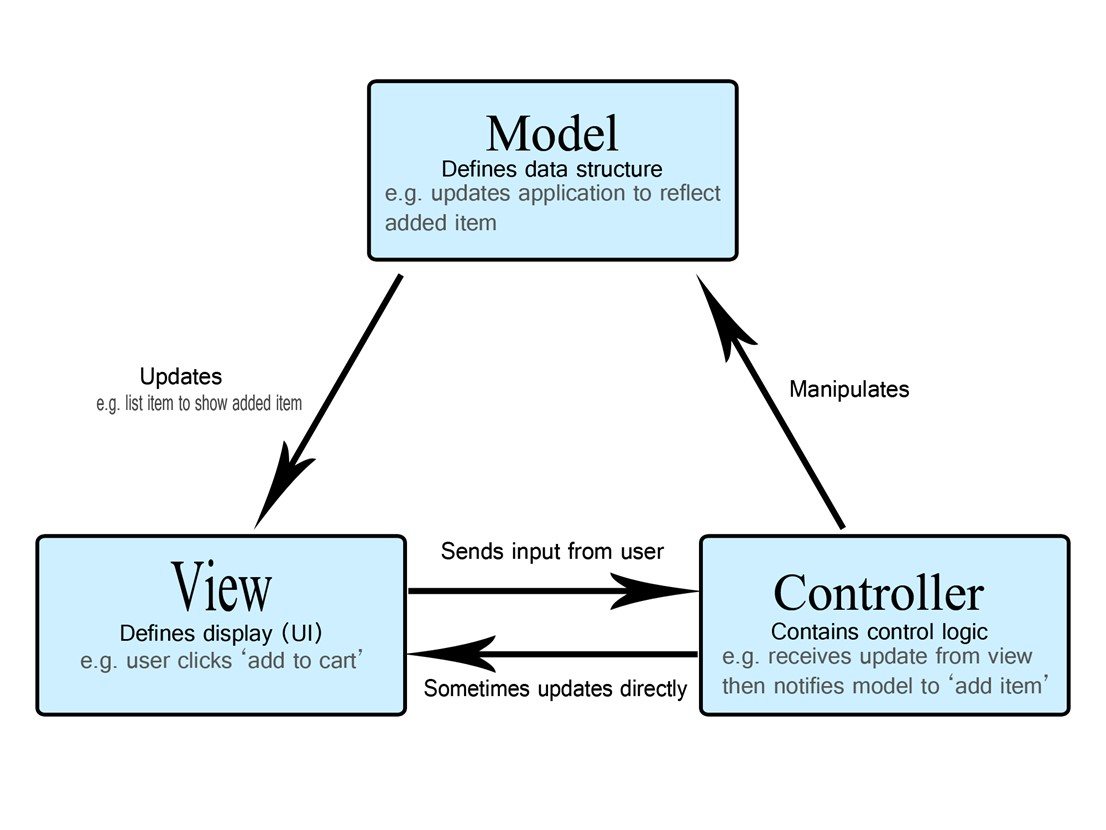
\includegraphics[width=10cm]{image/mvc.jpg} 
\caption{ภาพแสดงหลักการของ MVC Architecture จาก \url{https://developer.mozilla.org/en-US/docs/Glossary/MVC}}
\label{fig:mvc}
\end{figure}

\item \textbf {Client-Server Model }
Client-Server Model [21] คือเป็นรูปแบบโครงสร้างของเว็บแอปพลิเคชันรูปแบบหนึ่งซึ่งประกอบไปด้วย 2 ส่วนได้แก่
\begin{itemize}
\item Client หรือ ผู้ขอใช้บริการหรือต้องการบริการบางอย่างจาก Server
\item Server หรือผู้ให้บริการ
\end{itemize}
รูปแบบโครงสร้าง Client-Server นั้นช่วยในเรื่องรองรับการเข้าถึงข้อมูลพร้อมๆกันในเวลาเดียวกัน[21] โดย Client จะส่ง Request ไปให้กับ Server ส่วน Server เปรียบเสมือนคนกลางที่คอยติดต่อกับ Database และประมวลผลข้อมูลต่างๆและส่งไปให้ Client ดังภาพ~\ref{fig:client}

\begin{figure}[!h]\centering
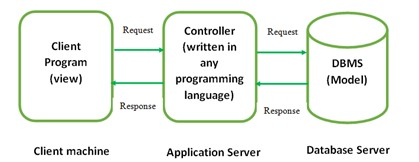
\includegraphics[width=10cm]{image/client.jpg} 
\caption{ภาพแสดงหลักการของ  MVC Architecture ใน Client-Server Model จาก \url{https://www.wideskills.com/struts/introduction-to-mvc-architecture}} 
\label{fig:client}
\end{figure}

\item \textbf {Proxy Server}
[22,23] เป็นตัวกลางคั่นกลางระหว่าง Client และ Server เพื่อไม่ให้ Client สามารถติดต่อโดยตรงกับ Server ได้ เพื่อเพิ่มความปลอดภัยให้กับ Server โดยสามารถป้องกัน Request ที่ไม่พึงประสงค์ได้ สามารถกำหนดสิทธิ์ในการเข้าถึง Serverได้ และยังเพิ่มประสิทธิภาพให้กับ Server อีกด้วยการ Cache เนื้อหาที่มีการมีการเข้าถึงบ่อยจึงสามารถเรียกใช้งานได้อย่างรวดเร็ว

\item \textbf {Object Relational Mapping (ORM)}
[25] เป็นการ map ข้อมูลใน Database ให้อยู่ในรูปแบบของ Object-Orient Language และแปลงจาก Object-Orient Language กลับไปเป็นข้อมูลที่เป็นรูปแบบข้อมูลที่มีความสัมพันธ์ได้ ทำให้เราเข้าถึงข้อมูลได้โดยไม่ต้องเขียน SQL แต่จะเข้าถึงผ่าน Object ที่สร้างขึ้นมาแทนองค์ประกอบของ ORM ซึ่งเป็นตัวกลางในการแปลงข้อมูล และสามารถรองรับการ Query ในรูปแบบต่างๆเพื่อรองรับกับความต้องการของนักพัฒนาได้

\end{itemize}

\section{ภาษาโปรแกรมและเทคโนโลยีที่ใช้ }

\subsection{ภาษาโปร}

\begin{enumerate}
\item \textbf{Typescript} เป็นส่วนขยายของ JavaScript ที่เพิ่มการระบุชนิดข้อมูลและสนับสนุนแนวคิดของ Object-Oriented Programming (OOP) เพื่อเพิ่มประสิทธิภาพและความคงทนในการพัฒนาโปรแกรม JavaScript ให้ดียิ่งขึ้น ทางคณะผู้จัดทำได้ใช้ในการพัฒนาเว็บแอปพลิเคชันทั้งในส่วนของ Front-End และ Back-End
\item \textbf{Python} เป็นภาษาโปรแกรมมิ่งระดับสูงที่มีความเข้าใจง่ายและมีความหลากหลายในการใช้งาน มันเป็นภาษาที่มีการเรียนรู้และการใช้งานที่สะดวก ทำให้เป็นที่นิยมอย่างมากในหลายสายงานและอุตสาหกรรมต่าง ๆ รวมถึงเป็นภาษาหลักที่ใช้ในงานด้าน Data Science และ Machine Learning [16] 
ทางคณะผู้จัดทำใช้ภาษา Python ในการพัฒนาและดัดแปลง Stable Diffusion ให้เหมาะสมกับโครงงาน	
\end{enumerate}

\subsection{เทคโนโลยี}
\hspace {18pt}ในการพัฒนาเว็บแอปพลิเคชันในส่วนต่าง ๆทางคณะผู้จัดทำได้ใช้ Next.js ในการพัฒนา Front-End ร่วมกับ TailwindCSS และได้ใช้ ExpressJS ในการพัฒนา Back-End ในส่วนของ Generative AI ของผู้จัดทำได้ใช้ Stable Diffusion ในการ Generate รูปภาพและได้ใช้เครื่องมือที่ชื่อว่า kohya เป็นเครื่องมือในการ Train โมเดล	

\begin{enumerate}

\item \textbf{Next.JS} เป็นเฟรมเวิร์กที่มี Server-Side Rendering (SSR) ที่ช่วยปรับปรุงประสิทธิภาพและ SEO ของเว็บไซต์ได้อย่างเหนือชั้น โดยสร้างและส่งเนื้อหา HTML จากเซิร์ฟเวอร์โดยตรง ทำให้เว็บแอปพลิเคชันโหลดแสดงข้อมูลเร็วและมีโอกาสอันดับสูงในผลการค้นหาของ Google และบราวเซอร์ต่าง ๆ นอกจากนี้ Next.js ยังสนับสนุน Pre-rendering เพื่อเพิ่มประสิทธิภาพในการโหลดและให้ประสบการณ์ผู้ใช้ที่ดี ทั้งนี้ Next.js เป็นโปรเจ็กต์ open-source ที่เกิดจากบริษัทเอกชน Vercel ที่มีชื่อเสียงในวงการเว็บโฮสติ้งและมีการพัฒนาและการรับรองจากชุมชนที่ใหญ่อย่างกว้างขวาง
\item \textbf{TailwindCSS} เป็นเฟรมเวิร์ก สำหรับสร้างสไตล์ CSS ของเว็บแอปพลิเคชัน มันเป็นโปรเจ็กต์ open-source ที่ออกแบบมาเพื่อช่วยให้การจัดรูปแบบเว็บไซต์เป็นเรื่องง่ายและมีประสิทธิภาพมากขึ้น วิธีการทำงานของ Tailwind CSS คือการนำคลาส (Class) ย่อยๆ ที่ถูกกำหนดไว้ล่วงหน้า มาใช้งานและรวมกันเพื่อสร้างสไตล์ตามที่ต้องการ
\item \textbf{ExpressJS} เป็นเฟรมเวิร์ก สำหรับพัฒนาแอปพลิเคชันเว็บและเว็บเซอร์วิสด้วย JavaScript ซึ่งใช้ Node.js เป็นพื้นฐาน มีความเร็วและประสิทธิภาพสูง รองรับการใช้งาน Middlewares และช่วยในการจัดการเริ่มต้นและสร้าง API อย่างง่าย ๆ ด้วยการสนับสนุนเส้นทางและคอนโทรลเลอร์ มีชุมชนและความร่วมมือจากนักพัฒนาทั่วโลก
\item \textbf{Stable Diffusion} เป็น Generative AI ที่เผยแพร่ในปี 2022 โดยใช้เทคนิค Diffusion มันใช้สำหรับสร้างรูปภาพที่ละเอียดโดยมีข้อความเป็นเงื่อนไข แต่ยังสามารถนำมาใช้ในงานอื่น ๆ เช่น inpainting, outpainting, และการสร้างภาพแปลงแปลงจากภาพอื่นๆ ตามคำบรรยายข้อความได้ด้วย โมเดลนี้ถูกพัฒนาโดยนักวิจัยจากกลุ่ม CompVis ที่มหาวิทยาลัย Ludwig Maximilian University of Munich และ Runway พร้อมทั้งการบริจาคเทคโนโลยีการประมวลผลจาก Stability AI และข้อมูลการฝึกจากองค์กรไม่แสวงหาผลกำไร โมเดล Stable Diffusion เป็นโมเดล Latent Diffusion ที่เป็นชนิดของ Deep Generative Artificial Neural Network โค้ดและน้ำหนักของโมเดลถูกเปิดเผยสู่สาธารณะและสามารถใช้งานบนคอมพิวเตอร์ ที่มี GPU ขนาดเล็กอย่างน้อย 8 GB VRAM ซึ่งทำให้สามารถเข้าถึงได้ง่ายมากกว่าโมเดลอื่นๆ เช่น Midjourney หรือ Dall ·E
\item \textbf{Kohya}เป็น GUI (Graphical user interface) สำหรับ Train Model ให้กับ Stable Diffusion ซึ่ง UI จะใช้ตั้งค่าพารามิเตอร์ในการ Train และรันคำสั่ง CLI (Command-line user interface) สำหรับการฝึกโมเดล

\end{enumerate}

\subsection{ระบบฐานข้อมูล}

\begin{enumerate}
\item \textbf{MongoDB} เป็น open source NoSQL Database จัดเก็บข้อมูลในรูปแบบ document ที่ยืดหยุ่นและสามารถขยายได้ มีความสามารถในการจัดเก็บข้อมูลแบบไม่มีโครงสร้างคงที่ทำให้เหมาะสำหรับข้อมูลที่ไม่มีโครงสร้างคงที่หรือเปลี่ยนแปลงบ่อย มีประสิทธิภาพสูงในการอ่านและเขียนข้อมูล มีภาษาคิวรีที่มีประสิทธิภาพและสนับสนุนการใช้งานที่หลากหลาย สร้างสรรค์เป็นอย่างดีสำหรับการจัดเก็บข้อมูลที่ยืดหยุ่นและใช้งานระบบที่มีปริมาณข้อมูลมากหรือโหลดการใช้งานสูง
\item \textbf{PostgreSQL} เป็น open source SQL Database ที่มีความมั่นคงและคุณสมบัติมากมาย มันเหมาะสำหรับการพัฒนาและจัดการข้อมูลในแอปพลิเคชันและโครงการต่าง ๆ โดยใช้ SQL สำหรับการสอบถามและจัดการข้อมูล มีความยืดหยุ่นและประสิทธิภาพสูง และมีระบบควบคุมความแข็งแกร่งเพื่อความเสถียร มันเป็นเครื่องมือที่มีความนิยมในการพัฒนาแอปพลิเคชันและโปรเจคที่ต้องการระบบฐานข้อมูลที่เชื่อถือได้และมีประสิทธิภาพ	
\item \textbf{Cloudinary} เป็นบริการคลาวด์สำหรับจัดการและเก็บสื่อดิจิทัล เช่น รูปภาพและวิดีโอ ซึ่งช่วยให้ผู้ใช้สามารถเรียกใช้และจัดการสื่อเหล่านี้ในแอปพลิเคชันหรือเว็บไซต์ของพวกเขาได้อย่างง่ายดาย รวมถึงการให้ความสามารถในการปรับขนาดและแก้ไขสื่อ รวมถึงการใช้ API เพื่อจัดการกับสื่อต่าง ๆ บนพื้นที่คลาวด์ของพวกเขา
\end{enumerate}

\subsection{เครื่องมือที่ใช้ในการจัดการเวอร์ชั่นและทดสอบ}

\begin{enumerate}
\item \textbf{Git} เป็นเครื่องมือที่ช่วยในการบริหารจัดการเวอร์ชั่นของโค้ด โดยการบันทึกประวัติการสร้าง/ลบ/แก้ไขไฟล์แต่ละไฟล์โดยผู้ใช้งานแต่ละคน พร้อมทั้งบันทึกข้อมูลเป็นประวัติการเปลี่ยนแปลงทั้งหมด ทำให้สามารถติดตามการแก้ไขโค้ดได้อย่างละเอียด และย้อนกลับไปในประวัติโค้ดได้ คุณสมบัตินี้เป็นประโยชน์มากในการทำงานทีมและช่วยให้การจัดการโค้ดเป็นไปอย่างเรียบร้อยและมีประสิทธิภาพ 
\item \textbf{Jenkins} เป็นเครื่องมือสำหรับทำงานอัตโนมัติ (Automation) ในกระบวนการพัฒนาซอฟต์แวร์ ช่วยในการสร้าง ทดสอบ และส่งมอบโค้ดโดยอัตโนมัติ ซึ่งเป็นประโยชน์ในการลดเวลาและความเสี่ยงในการพัฒนาซอฟต์แวร์ Jenkins สามารถใช้งานได้กับหลายภาษาและแพลตฟอร์ม และมีหลายปลั๊กอินที่ช่วยในการปรับแต่งและขยายความสามารถของมัน ส่งผลให้ Jenkins เป็นเครื่องมือยอดนิยมสำหรับ Continuous Integration และ Continuous Deployment (CI/CD) ในกระบวนการพัฒนาซอฟต์แวร์
\end{enumerate}

\chapter{วิธีการทำงาน กระบวนการและการออกแบบ}

\section{บทนำ}
\hspace {18pt} ในบทที่ 3 จะกล่าวถึงโครงงานของเราจะมีวิธีการทำงานอย่างไร โครงสร้างทางระบบที่ทางเราได้วางเอาไว้ การใช้งานหว่างระบบออกแบบมาตอบโจทย์ผู้ใช้งาน รวมถึงการจัดการระบบที่ออกแบบมา และผลตอบรับจากแบบสอบถามที่ผู้จัดได้ทำขึ้นหาเพื่อวิเคราะห์ความต้องการของผู้ใช้งาน

\section{วิเคราะห์ความต้องการ}
\hspace {18pt} คณะผู้จัดทำได้สำรวจ Requirement จากการทำแบบสอบถามโดยมีผู้ทำแบบสอบถาม 50 คน และคณะผู้จัดทำสามารถวิเคราะห์จากผลตอบรับได้ดังนี้

\begin{figure}[!h]\centering
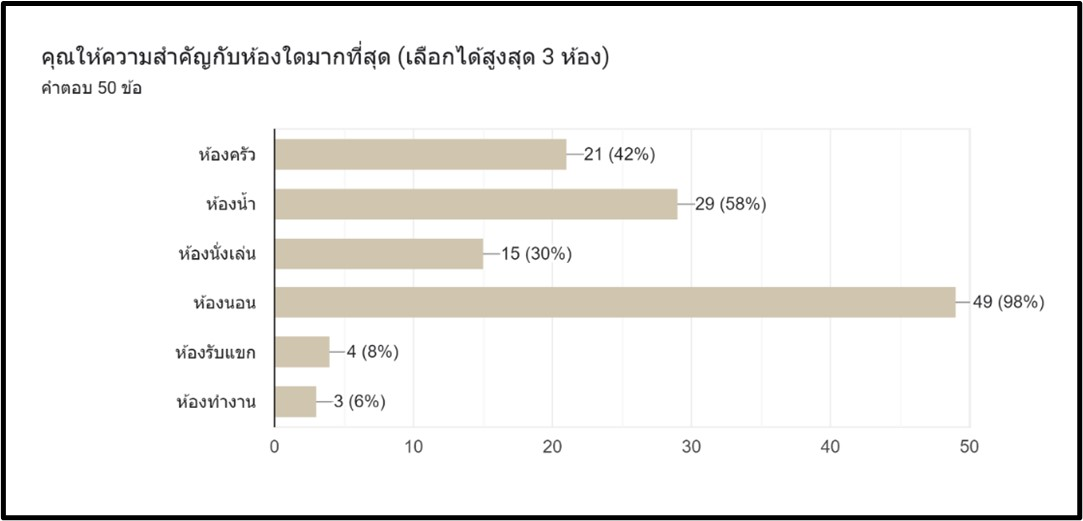
\includegraphics[width=10cm]{image/requirement.jpg}
\caption{แผนภูมิแสดงความคิดผู้ทำแบบสอบถามถึงความสำคัญห้องประเภทใดมากที่สุด}
\label{fig:requirement}
\end{figure}

\begin{figure}[!h]\centering
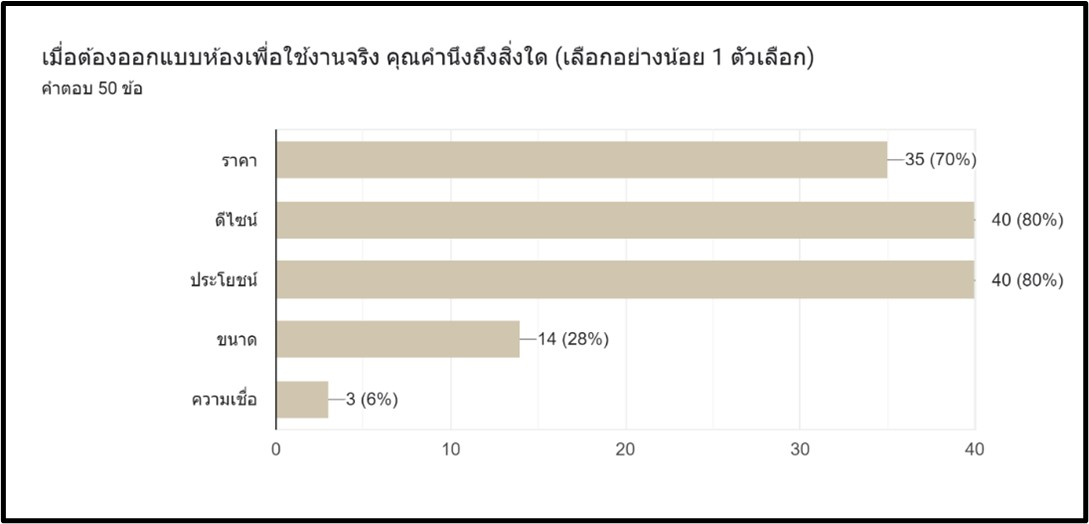
\includegraphics[width=10cm]{image/requirement-2.jpg}
\caption{แผนภูมิแสดงสิ่งที่ผู้ทำแบบสอบถามคำนึงหากต้องออกแบบห้องเพื่อใช้งานจริง}
\label{fig:requirement-2}
\end{figure}

\hspace {18pt} จากผลการตอบรับในภาพ~\ref{fig:requirement} ทำให้ทางคณะผู้จัดทำพบว่าห้องนอนมีความสำคัญมากที่สุด รองลงมาคือห้องน้ำและห้องนั่งเล่นเป็นอันดับที่สาม และจากภาพ~\ref{fig:requirement-2} คณะผู้จัดทำพบว่าดีไซน์และประโยชน์มีความสำคัญมากที่สุดและรองลงมาคือราคาและขนาดเป็นอันดับที่สาม จากผลการตอบรับดังกล่าว คณะผู้จัดทำจึงได้ข้อสรุปว่าจะพัฒนาเว็บแอปพลิเคชันให้สามารถใช้งานได้กับห้อง 3 ประเภทดังนี้ 1.ห้องนอน 2.ห้องน้ำ 3.ห้องครัว และเนื่องจากประโยชน์นั้นเป็นตัวชี้วัดที่ไม่ชัดเจน คณะผู้จัดทำตัดสินใจที่จะพัฒนาเว็บแอปพลิเคชันให้สามารถระบุทั้งราคาโดยรวมและดีไซน์ของห้อง

%%%%%%%%%%%%%%%%% Move to the next page %%%%%%%%%%%%%%%%
\vspace{\fill}\clearpage

\begin{figure}[!h]\centering
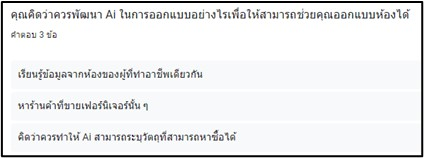
\includegraphics[width=10cm]{image/requirement-3.jpg}
\caption{แสดงถึงความคิดเห็นของผู้ทำแบบสอบถามในคำถามที่ว่าควรพัฒนา AI ในการออกแบบอย่างไรเพื่อให้สามารถช่วยในการออกแบบห้องได้}
\label{fig:requirement-3}
\end{figure}

\hspace {18pt}จากภาพ~\ref{fig:requirement-3} คณะผู้จัดได้ข้อสรุปว่าควรพัฒนาระบบให้สามารถสร้างรูปภาพโดยประกอบไปด้วยผลิตภัณฑ์ที่มีตัวแทนจำหน่ายในประเทศไทยเท่านั้น เช่น Index Living Mall Homepro ไทวัสดุ และ SB Design Square และพัฒนาเว็บแอปพลิเคชันให้สามารถตรวจจับเฟอร์นิเจอร์พร้อมทั้งระบุแหล่งจัดจำหน่าย

\begin{figure}[!h]\centering
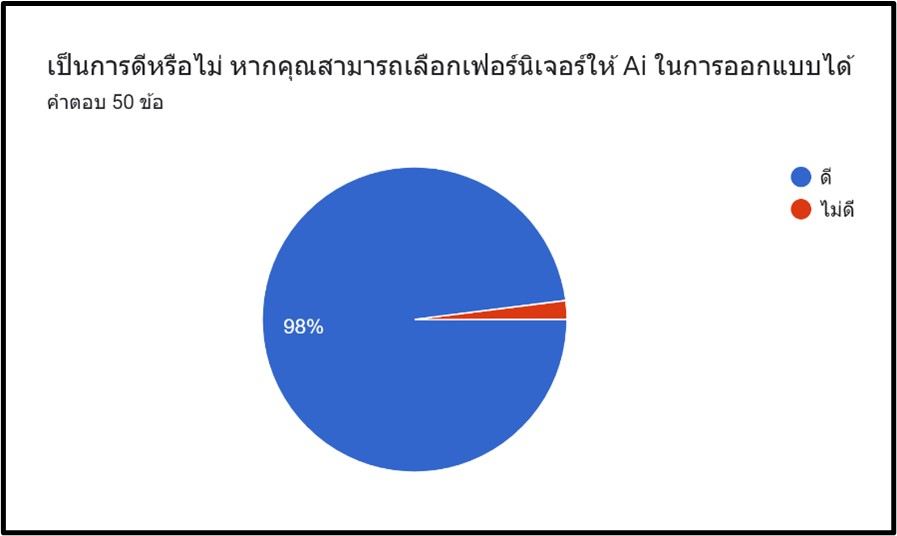
\includegraphics[width=10cm]{image/requirement-4.jpg}
\caption{แสดงถึงความคิดเห็นของผู้ทำแบบสอบถามว่าจะเป็นการดีหรือไม่ หากคุณสามารถเลือกเฟอร์นิเจอร์ให้ AI ในการออกแบบได้}
\label{fig:requirement-4}
\end{figure}

\begin{figure}[!h]\centering
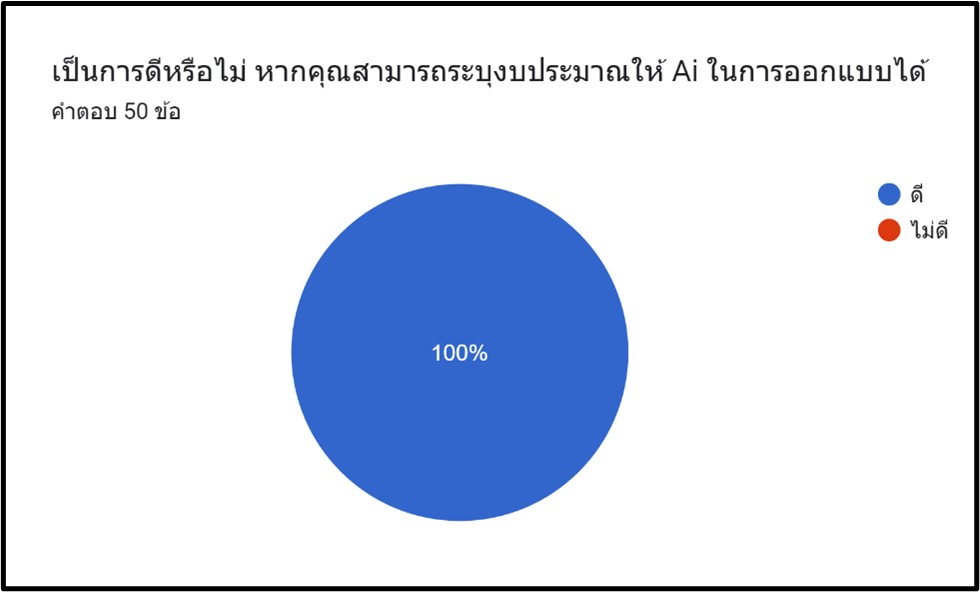
\includegraphics[width=10cm]{image/requirement-5.jpg}
\caption{แสดงถึงความคิดเห็นของผู้ทำแบบสอบถามว่าจะเป็นการดีหรือไม่ หากคุณสามารถระบุงบประมาณให้ AI ในการออกแบบได้}
\label{fig:requirement-5}
\end{figure}

%%%%%%%%%%%%%%%%% Move to the next page %%%%%%%%%%%%%%%%
\vspace{\fill}\clearpage

\begin{figure}[!h]\centering
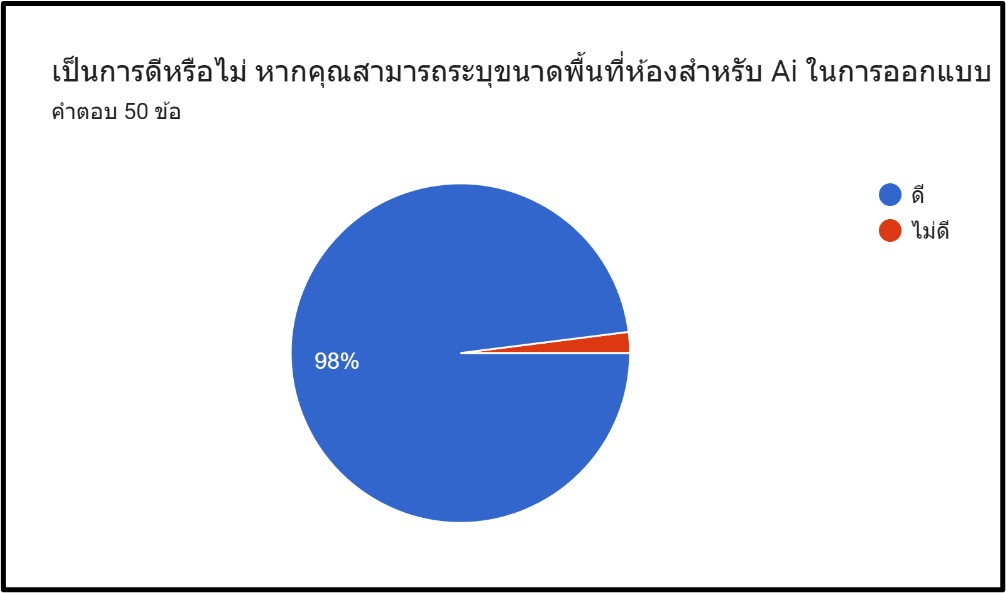
\includegraphics[width=10cm]{image/requirement-6.jpg}
\caption{แสดงถึงความคิดเห็นของผู้ทำแบบสอบถามว่าจะเป็นการดีหรือไม่ หากคุณสามารถระบุขนาดพื้นที่ห้องสำหรับ AI ในการออกแบบ}
\label{fig:requirement-6}
\end{figure}

\begin{figure}[!h]\centering
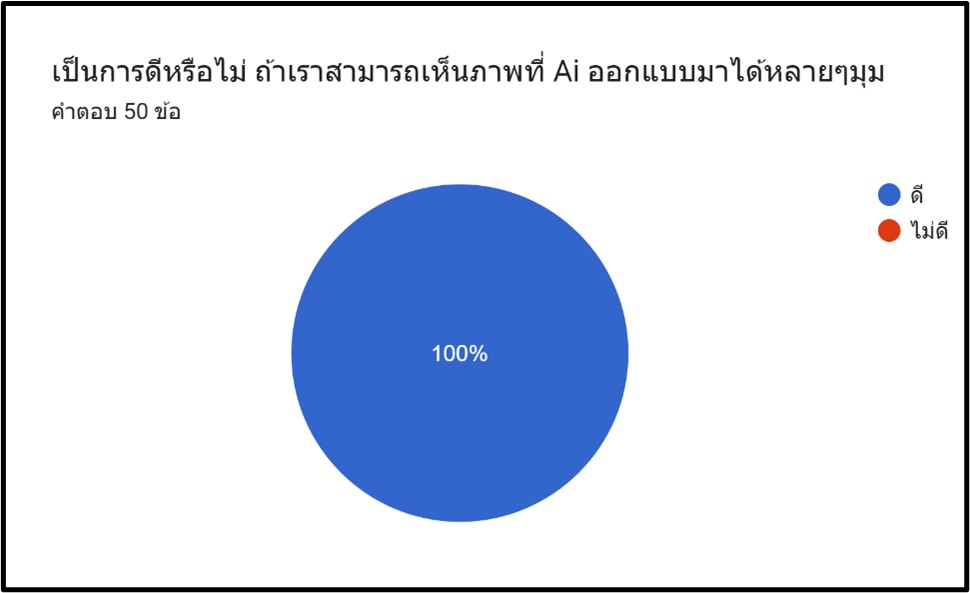
\includegraphics[width=10cm]{image/requirement-7.jpg}
\caption{แสดงถึงความคิดเห็นของผู้ทำแบบสอบถามว่าจะเป็นการดีหรือไม่ ถ้าเราสามารถเห็นภาพที่ AI ออกแบบมาได้หลายๆมุม}
\label{fig:requirement-7}
\end{figure}

%%%%%%%%%%%%%%%%% Move to the next page %%%%%%%%%%%%%%%%
\vspace{\fill}\clearpage

\begin{figure}[!h]\centering
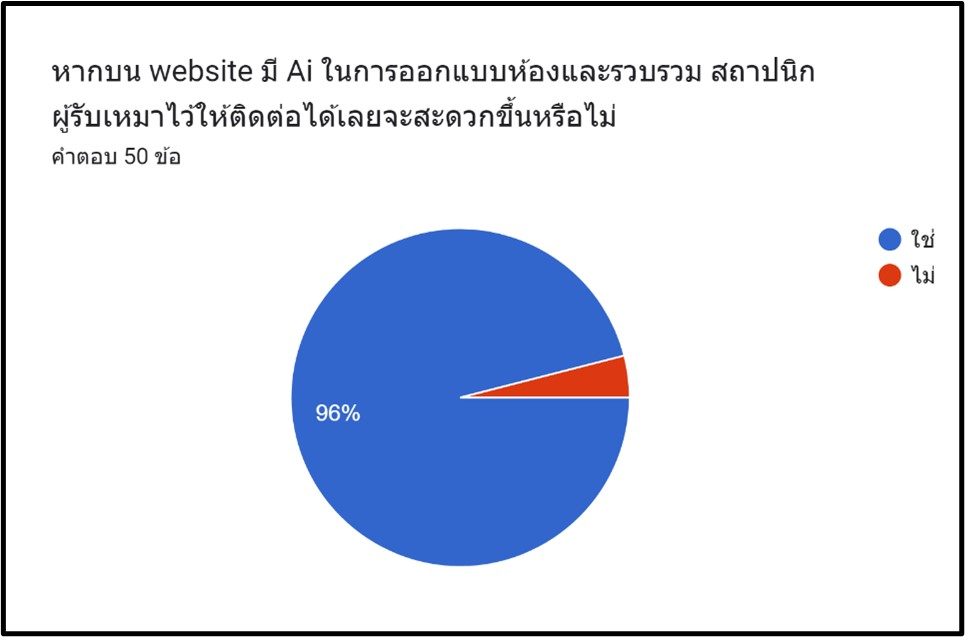
\includegraphics[width=10cm]{image/requirement-8.jpg}
\caption{แสดงถึงความคิดเห็นของผู้ทำแบบสอบถามถึงคำถามหากบน Website มี AI ในการออกแบบห้องและรวบรวม สถาปนิก ผู้รับเหมาไว้ให้ติดต่อได้เลยจะสะดวกขึ้นหรือไม่}
\label{fig:requirement-8}
\end{figure}



จากแผนภูมิที่ ~\ref{fig:requirement-4} ~\ref{fig:requirement-5} ~\ref{fig:requirement-6}~\ref{fig:requirement-7} ~\ref{fig:requirement-8} คณะผู้จัดทำได้ทำการพิจารณาและวิเคราะห์ความเป็นไปได้ซึ่งคณะผู้จัดทำได้ข้อสรุปดังนี้ 

\begin{enumerate}
\item คณะผู้จัดทำจะพัฒนาเว็บแอปพลิเคชันให้ผู้ใช้สามารถเลือกเฟอร์นิเจอร์หรือผลิตภัณฑ์ให้ AI สร้างรูปภาพห้องที่มีเฟอร์นิเจอร์ที่ผู้ใช้เลือก
\item คณะผู้จัดทำจะพัฒนาเว็บแอปพลิเคชันให้ผู้ใช้สามารถระบุงบประมาณของเฟอร์นิเจอร์โดยรวมให้ AI สร้างรูปภาพห้อง
\item คณะผู้จัดทำตัดสินใจที่จะไม่พัฒนาเว็ปแอปพลิเคชันให้ผู้ใช้สามารถระบุขนาดพื้นที่ห้องให้กับ AI เนื่องจากไม่มีเวลาเพียงพอและเป็นที่เรื่องที่ซับซ้อนในการพัฒนา 
\item คณะผู้จัดทำตัดสินใจที่จะไม่พัฒนาเว็ปแอปพลิเคชันให้สามารถสร้างรูปภาพในหลากหลายมุมมอง เช่น Top View Front View Side View เนื่องจากมีความซับซ้อนในการพัฒนา 
\item คณะผู้จัดทำตัดสินใจที่จะไม่พัฒนาเว็บแอปพลิเคชันให้สามารถติดต่อสถาปนิกและผู้รับเหมา เนื่องจากการปรับเปลี่ยนขอบเขตของงาน จึงทำให้ความสำคัญของสิ่งนี้ลดน้อยลง
\end{enumerate}

\section{รายละเอียดโครงงาน}
\hspace {18pt} ในโครงการนี้จะทำเว็บแอปพลิเคชันที่ใช้โมเดลที่ผ่านการ train มาแล้วรับคำสั่ง prompt แล้วนำไปสร้างห้องพร้อมตกแต่งภายในรวมไปถึงระบุสิ่งของที่ใช้ภายในห้องๆนั้นพร้อมกับประเมินราคาเพื่อให้ผู้ใช้ที่มีความต้องการจะใช้ปัญญาประดิษฐ์ในการออกแบบภายในและต้องการทราบค่าใช้จ่ายในการก่อสร้างรวมไปถึงทราบรายละเอียดของตกแต่งต่าง ๆ

\subsection{รายละเอียดโครงงาน}

\begin{itemize}
\item \textbf{Client} คอมพิวเตอร์ที่สามารถเล่นอินเทอร์เน็ตได้
\item \textbf{Server} 
\begin{itemize}
\item GPU: Nvidia geforce graphics card
\item VRAM: 10 GB or higher
\item Storage: 12 GB or higher
\item OS: Windows, MacOS or linux [14]
\end{itemize}
\end{itemize}

\subsection{Use cases}
\hspace {18pt}ผู้ใช้ที่มีความต้องการเครื่องมืออำนวยความสะดวกในเรื่องของการออกแบบภายในและต้องการทราบราคาที่ใช้ในการก่อสร้างรวมไปถึงรายละเอียดสิงของต่างๆ อาทิเช่น ราคา สถานที่จำหน่าย เพื่อเพิ่มความสะดวกสบายในการค้นหาสินค้าตกแต่งบ้าน โดย Guest สามารถที่จะ Login และ Register Customer สามารถที่จะใช้ AI ในการสร้างรูปภาพ ดูรูปภาพที่ตนให้ AI สร้าง สามารถดูประวัติการใช้งานของตน สามารถอัปโหลดรูปภาพให้ AI ในการค้นหาผลิตภัณฑ์ที่มีในเว็บไซต์ และ Admin สามารถทำทุกอย่างที่ Customer ทำได้ทั้งหมด และสิ่งที่ทำได้เพิ่มเติมดังนี้ สามารถดูข้อมูลการใช้เฟอร์นิเจอร์ของ AI ในการสร้างรูปภาพ อัตราการใช้แต่ละสไตล์และชนิดของห้องของผู้ใช้งานซึ่งจะอยู่ในรูปแบบของ Dashboard และสามารถเพิ่มผลิตภัณฑ์และเฟอร์นิเจอร์ได้ ดังภาพ~\ref{fig:use-case}

\begin{figure}[!h]\centering
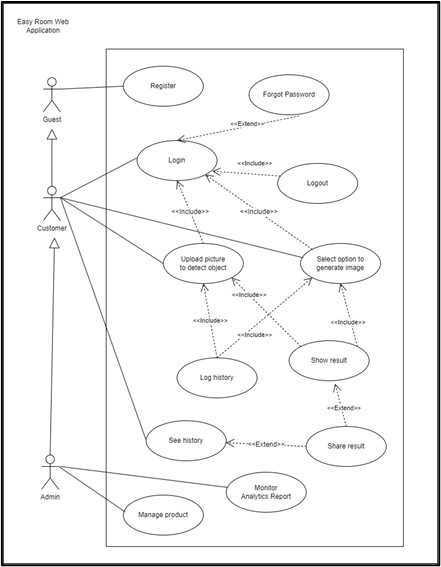
\includegraphics{image/use-case.jpg}
\caption{Use Case Diagram}
\label{fig:use-case}
\end{figure}

%%%%%%%%%%%%%%%%% Move to the next page %%%%%%%%%%%%%%%%
\vspace{\fill}\clearpage

\subsection{Workflow}
\hspace {18pt}ในเว็บแอปพลิเคชันมีโมเดลที่ถูกtrainมาแล้วโดยผู้ใช้สามารถกรอกข้อมูลตามที่พวกเรากำหนดจากนั้นจะส่งข้อมูลเข้าไปประมวลผลในโมเดลแล้วจะแสดงรูปภาพพร้อมทั้งผลิตภัณฑ์และมูลค่าโดยประมาณของผลิตภัณฑ์ที่ใช้ในภาพให้กับผู้ใช้ ดังภาพ~\ref{fig:sequence} ลำดับกระบวนการทำงานในการสร้างรูปภาพ 

\begin{figure}[!h]\centering
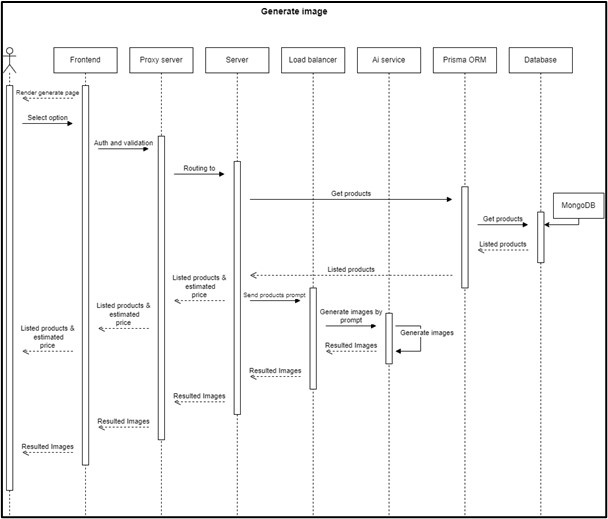
\includegraphics{image/sequence.jpg}
\caption{Sequence Diagram}
\label{fig:sequence}
\end{figure}

%%%%%%%%%%%%%%%%% Move to the next page %%%%%%%%%%%%%%%%
\vspace{\fill}\clearpage

\begin{figure}[!h]\centering
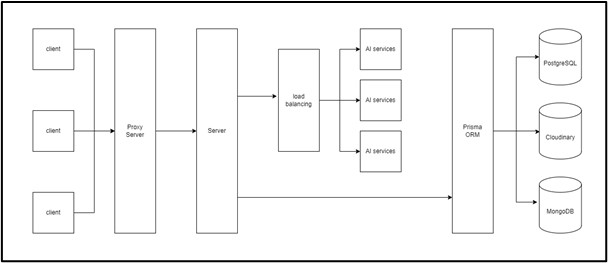
\includegraphics{image/system.jpg}
\caption{System Diagram}
\label{fig:system}
\end{figure}

\hspace {18pt}จากภาพ~\ref{fig:system} สามารถอธิบายได้ว่า Client จะไม่สามารถติดต่อสื่อสารโดยตรงกับ Server ได้จะต้องติดต่อผ่าน Proxy Server เท่านั้นเพื่อเพิ่มความปลอดภัยให้มากขึ้น โดยในส่วนนี้จะมีการยืนยันตัวตนให้กับผู้ใช้ และทำการตรวจสอบข้อมูลก่อนทีจะส่งไปยัง Server และ Request ที่ต้องการใช้งานในส่วนของ AI จะถูกส่งไปยัง Load Balancer เพื่อทำการจัดคิวการเข้าใช้งานของ GPU (ณ ตอนนี้ Client ยังไม่สามารถใช้งาน AI ได้พร้อมกันเนื่องจากมีข้อจำกัดทางฮาร์ดแวร์คือ GPU ไม่เพียงพอต่อการใช้งาน) 

\hspace {18pt}เนื่องจากเว็บแอปพลิเคชัน Easy Room ได้มีการใช้ Database ที่มีความหลากหลายไปตามความสามารถจึงเลือกที่จะใช้ Prisma ORM เพื่อเป็นตัวกลางในการติดต่อสารระหว่าง Server กับ Database เพื่อลดความภาระของการศึกษาการเรียกใช้งานของแต่ละ Database

%%%%%%%%%%%%%%%%% Move to the next page %%%%%%%%%%%%%%%%
\vspace{\fill}\clearpage

\subsection{Database ER diagram}

\begin{figure}[!h]\centering
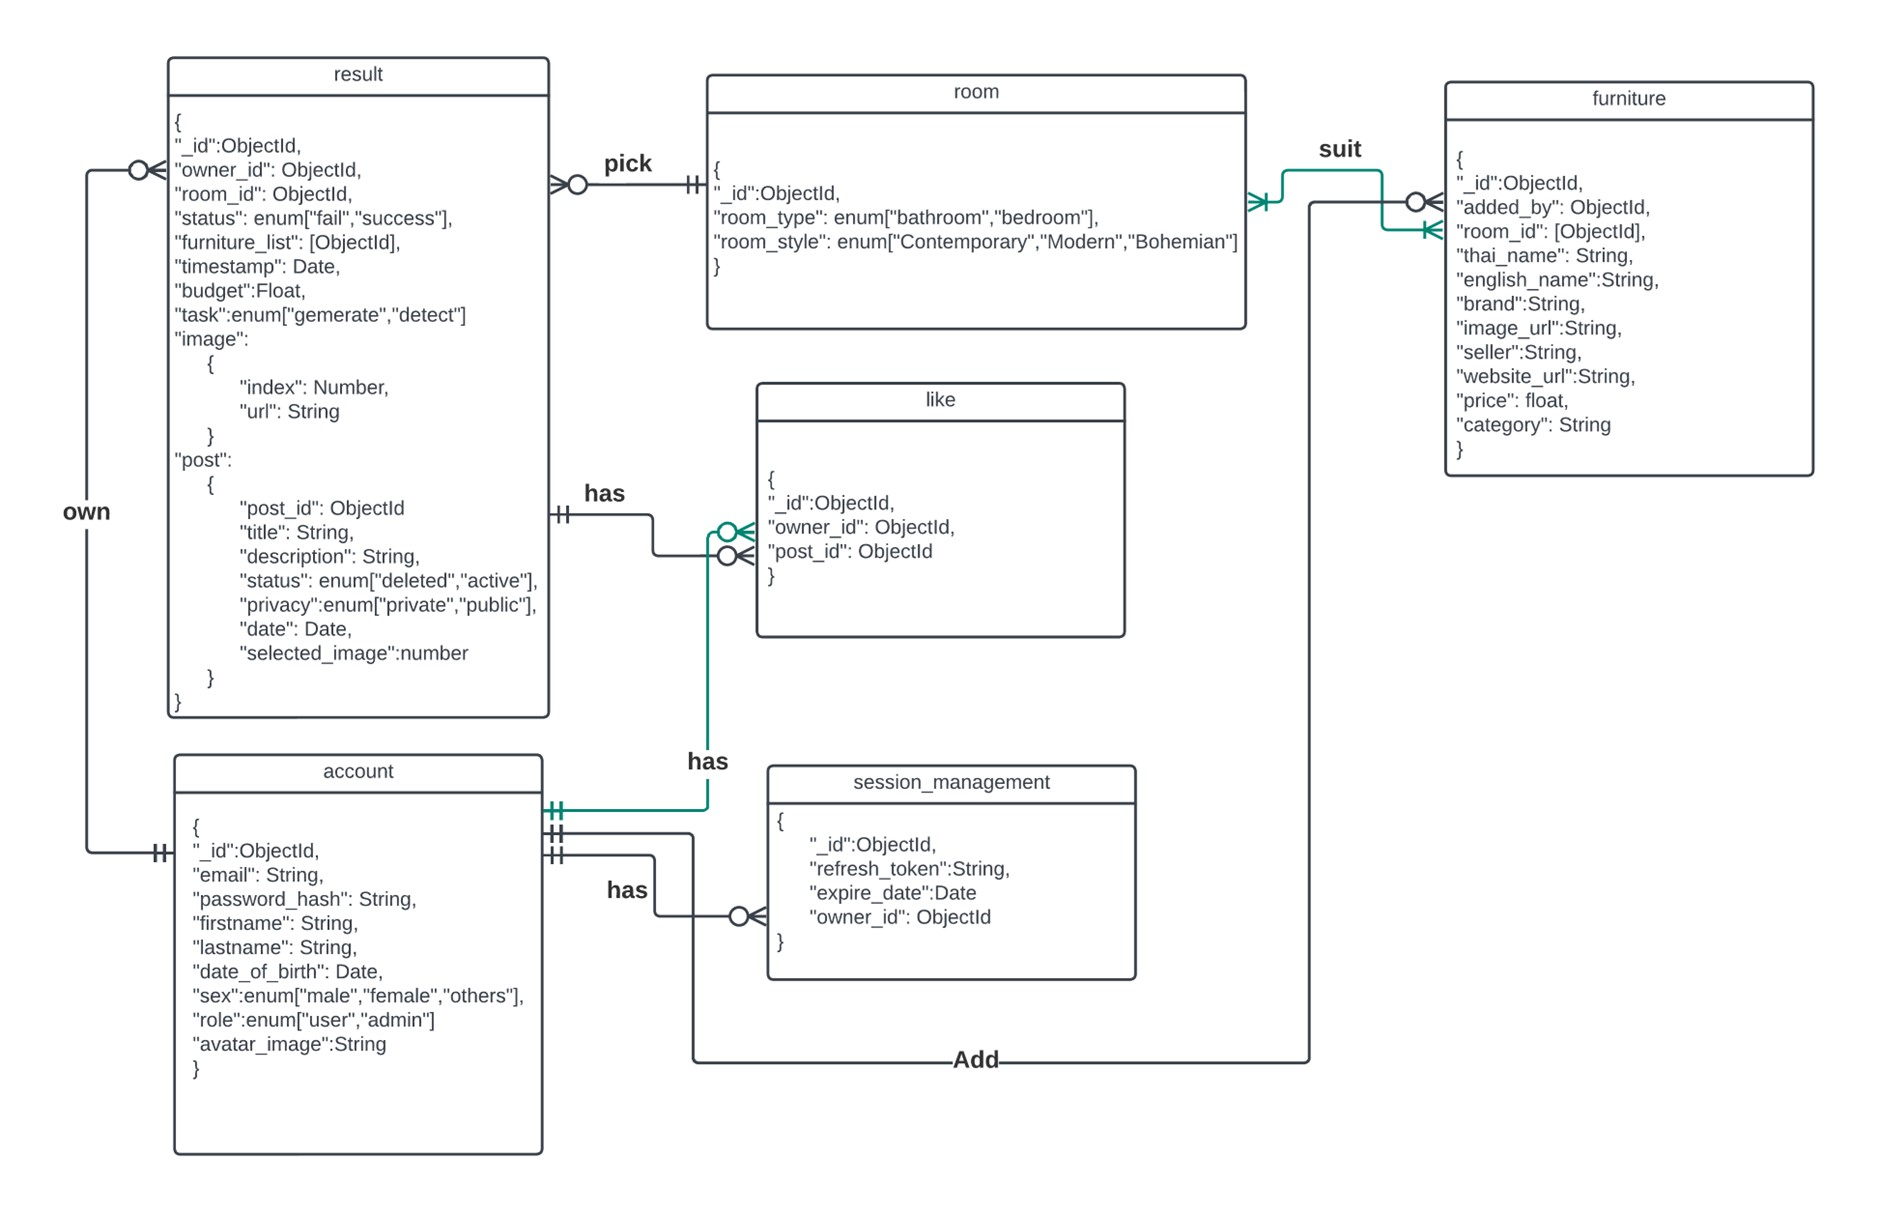
\includegraphics{image/er.jpg}
\caption{ER Diagram}
\label{fig:er}
\end{figure}

\hspace {18pt} จากภาพ~\ref{fig:er} สามารถบ่งบอกได้ว่าโครงสร้างของ Database ของเว็บแอปพลิเคชัน Easy Room มีทั้งหมด 6 collections คือ 1.account 2.result 3.session\_management 4.like 5.room และ 6.furniture ซึ่ง account จะมีหน้าที่ในการเก็บข้อมูลของผู้ใช้ โดยจะมี data dictionary ดังนี้




%%%%%%%%%%%%%%%%%%%%%%%%%%%%%%%%%% Ref %%%%%%%%%%%%%%%%%%%%%%%%%%%%%%%%%%%
\makeatletter
\g@addto@macro{\UrlBreaks}{\UrlOrds}
\makeatother
% 

\bibliographystyle{kmutt}
\bibliography{string,cpe}

%%%%%%%%%%%%%%%%%%%%%%%%%%%%%%%%%%%%%%%%%%%%%%%%%%%%%%%%%%%%%%%
%%%%%%%%%%%%%%%%%%%%%%%% Appendix %%%%%%%%%%%%%%%%%%%%%%%%%%%%%
%%%%%%%%%%%%%%%%%%%%%%%%%%%%%%%%%%%%%%%%%%%%%%%%%%%%%%%%%%%%%%%
\appendix{แบบสอบถามสำหรับการวิเคราะห์ความต้องการ}
\noindent{\large\bf แบบสอบถามสำหรับการวิเคราะห์ความต้องการ} \\

\textbf{เรื่อง} ปัญญาประดิษฐ์ด้านการออกแบบภายใน

\hspace {18pt} แบบสอบถามนี้จัดทำขึ้นโดย นายธัญพิสิษฐ์ พิสิฐพล นายพฤฒิพล จิตรเจริญกิจ และนายวิชยุฒม์ 
ช่วยชูกูล นักศึกษาชั้นปีที่ 4 ภาควิชาวิศวกรรมคอมพิวเตอร์ มหาวิทยาลัยเทคโนโลยีพระจอมเกล้าธนบุรี

\hspace {18pt}มีจุดประสงค์เพื่อศึกษาและรวบรวมข้อมูลและความต้องการต่างๆ ในการใช้งาน AI ในงานออกแบบภายใน เพื่อใช้เป็นแนวทางในการพัฒนาระบบที่ช่วยอำนวยความสะดวกเกี่ยวกับการออกแบบภายใน โดยเราจะนำข้อมูลนั้นไปใช้ในการสร้างเว็บไซต์แอปพลิเคชันที่สามารถใช้งาน AI ในการสร้างรูปของห้องต่างๆและสามารถประเมินค่าใช้จ่ายทั้งหมดจากภาพที่ AI สร้างขึ้น ซึ่งข้อมูลที่ได้รับจะไม่ถูกนำไปเปิดเผยและใช้เพื่อการศึกษาเท่านั้น 

\hspace {18pt} สามารถเข้าทำแบบสอบถามได้จาก \url{https://forms.gle/jPAt6VJqqN2smsn29}







\end{document}
